% !TEX root = ../thesis.tex
% testing and optimization experiments
% @author Tobias Wulf
%

\chapter{Erprobungs- und Optimierungsexperimente}\label{ch:erprobungs-u-opt-exp}


In diesem Teil der Arbeit werden Experimente bzw. Simulationen durchgeführt, die abschnittweise Beiträge für eine Modelloptimierung zeigen. Dabei ist das übergeordnete Ziel ein möglichst ressourcenarmes mathematisches Modell für einen Sensor-ASIC zu finden. Die Durchführung der Experimente basiert auf Matlab-Skripten, in denen geschriebener funktionaler Quellcode eingebunden und ausgeführt wird. Die Ergebnisse der Experimente stehen nach Durchführung in Vektor- und Matrixform im Matlab-Workspace bereit und sind anschließend mit grafisch Ausgewertet worden. Die Ergebnisgrafiken sind unter den einzelnen Experimenten einzusehen, beschrieben und feststellend ausgewertet. Eine zusammenfassende Auswertung aller Ergebnisse folgt in \autoref{ch:zusammenfassung}. Der grundlegende Ablauf der Experimente ist schematisch gleich:


\begin{enumerate}
	\item Konfigurieren der Software und Erstellen der Konfigurations-MAT-Datei.
	\item Erzeugen von Trainings- und Testdatensätze mittels der Sensor-Array-Simulation.
	\item Erstellen eines oder mehrerer Regressionsmodell.
	\item Durchführung von Regressions- oder Verlustberechnungen.
	\item Grafische Auswertung der Ergebnisse.
\end{enumerate}


Als Grundparametrierung der Experimente dient die \autoref{tab:sim-params-exp}. Abweichende Parameter in den Experimenten sind gesondert aufgeschlüsselt. Die einzelnen Experimente werden nach Zweck, Durchführung, erzeugte Trainings- bzw. Testdatensätze, genutztes Matlab-Skript, abweichende Parametrierung von \autoref{tab:sim-params-exp}, Ergebnisse und Beobachtungen beschrieben. Die Experimente sind in Matlab-Skripten aus \autoref{mcode:executable-scripts} als ausführbarer Quellcode realisiert.


\clearpage


\begin{table}[htp]
	\centering
	\resizebox{\textwidth}{!}{
		\begin{tabular}{l l c c l}
			\toprule
			\textbf{Parametergruppe}                 & \textbf{Parameter}  & \textbf{Wert}        & \textbf{Einheit}  & \textbf{Kurzbeschreibung}                                           \\ \midrule
			\multirow{6}{*}{SensorArrayOptions}      & geometry            & 'square'             & -                 & Array-Geometrie-Indikator                                           \\
			                                         & dimension           & $8$                  & -                 & Sensor-Array-Pixel $N_{Pixel} \times N_{Pixel}$                     \\
			                                         & edge                & $2$                  & mm                & Sensor-Array-Kantenlänge                                            \\
			                                         & $V_{cc}$            & $5$                  & V                 & Sensor-Array-Betriebsspannung                                       \\
			                                         & $V_{off}$           & $2,5$                & V                 & Sensor-Brücken-Offset-Spannung                                      \\
			                                         & $V_{norm}$          & $1 \cdot 10^3$       & mV                & Kennfeldnormierung                                                  \\ \hline
			\multirow{4}{*}{DipoleOptions}           & sphereRadius        & $2$                  & mm                & Kugelmagnetradius                                                   \\
			                                         & $H_{0mag}$          & $200$                & $\text{kAm}^{-1}$ & Betragsfeldstärke Magnetfeldnormierung                              \\
			                                         & $z_0$               & $1$                  & mm                & $Z$-Abstand Magnetfeldnormierung                                    \\
			                                         & $m_{0mag}$          & $1 \cdot 10^6$       & $\text{Am}^2$     & Magnitude d. mag. Moments                                           \\ \hline
			\multirow{10}{*}{Training-/ TestOptions} & useCase             & 'Training'/ 'Test'   & 'char'            & Datensatzindikator f. Anwendungszweck                               \\
			                                         & xPos                & $\left[0,\right]$    & mm                & Sensor-Array $X$-Positionsvektor                                    \\
			                                         & yPos                & $\left[0,\right]$    & mm                & Sensor-Array $Y$-Positionsvektor                                    \\
			                                         & zPos                & $\left[7,\right]$    & mm                & Sensor-Array $Z$-Positionsvektor                                    \\
			                                         & tilt                & $0$                  & $^\circ$          & Magnetverkippung in $Y$-Achse                                       \\
			                                         & angleRes            & $0,5$                & $^\circ$          & Winkelauflösung f. Magnetrotation                                   \\
			                                         & phaseIndex          & 0                    & -                 & Phasenverschiebung-Index f. Startwinkel                             \\
			                                         & nAngles             & $20$/ $720$          & -                 & Anzahl gleich verteilter Simulationswinkel                          \\
			                                         & BaseReference       & 'TDK'                & char              & Kennfelddatensatzindikator                                          \\
			                                         & BridgeReference     & 'Rise'               & char              & Kennfeldindikator                                                   \\ \hline
			\multirow{10}{*}{GPROptions}             & kernel              & 'QFC'                & char              & Kernel-Funktion-Indikator \eqref{eq:kfun}, 'QFC' $\leftarrow d_F^2$ \\
			                                         & $\theta$            & $(1,1)$              & -                 & Kernel-Parametervektor $\theta$ \eqref{eq:kparam}                   \\
			                                         & $\sigma_f^2$-Bounds & $(0.1, 100)$         & -                 & Parameter-Bounds $\theta_1$ f. \autoref{alg:fminconopt}             \\
			                                         & $\sigma_l$-Bounds   & $(0.1, 100)$         & -                 & Parameter-Bounds $\theta_2$ f. \autoref{alg:fminconopt}             \\
			                                         & $\sigma_n^2$        & $10^{-6}$            & -                 & Rauschniveau, Rauschaufschaltung \eqref{eq:addnoise}                \\
			                                         & $\sigma_n^2$-Bounds & $(10^{-8}, 10^{-4})$ & -                 & Parameter-Bounds $\sigma_n^2$ f. \autoref{alg:bayesopt}             \\
			                                         & OptimRuns           & $30$                 & -                 & Durchlaufanzahl f. \autoref{alg:bayesopt}                           \\
			                                         & SLL                 & 'SLLA'               & char              & Verlust-Indikator f. Winkel (A)/ R (Radius) \autoref{alg:bayesopt}  \\
			                                         & mean                & 'zero'               & char              & Indikator Mittelwertpolynom Ein ('poly')/ Aus ('zero')              \\
			                                         & polyDegree          & $1$                  & -                 & Grad des Mittelwertpolynoms wenn mean = 'poly'                      \\ \bottomrule
		\end{tabular}}
	\caption[Simulationsparameter der Erprobungs- und Optimierungsexperimente]{Simulationsparameter der Erprobungs- und Optimierungsexperimente. Von der Grundparametrierung abweichende Werte werden direkt unter den jeweiligen Experimenten aufgeführt. Parametergruppen entsprechen dem Konfigurationsskript im \autoref{mcode:generateconfigmat}. Zusammenführung der \autoref{tab:sensor-array-sim-params} und \autoref{tab:gpr-sim-params}}
	\label{tab:sim-params-exp}
\end{table}


% !TEX root = ../thesis.tex
% compare covariance functions and generalization
% @author Tobias Wulf
%

\section{Vergleich der Kovarianzfunktionen und einsetzende Generalisierung}\label{sec:exp1}

\textbf{Zweck:} Als Vergleich der beiden implementierten Kernel-Module sollen ihre Kovarianzfunktionen und Eigenschaft zur Generalisierung bei einfacher Parametrierung untersucht werden. Ziel ist es, im besten Fall die Implementierung über die euklidische Abstandsfunktion nutzen zu können. Es würde sich dadurch eine Ressourcenersparnis in Bezug auf Speicherkapazität einstellen, da sich mit diesen Kernel Modelltrainingsdaten aus zwei eindimensionalen Vektoren bilden, statt dreidimensionaler Matrizen für die Kernel-Implementierung aus den Vorarbeiten. Diese nutzt als Abstandsfunktion die Frobenius Norm, siehe \autoref{eq:kfun}.


\clearpage


\textbf{Durchführung:} Es werden beide Kernel-Module nacheinander im Skript geladen und mit variierenden Parametern initialisiert. Die resultierenden Modelle werden ohne weitere Optimierungen betrieben, um grundlegende Eigenschaften der Kovarianzfunktionen und Generalisierung miteinander vergleichbar zu machen. Dabei wird eine Trainingsdatensatz verwendet der eine relative hohe Anzahl an Trainingspunkten $>50$ besitzt, dass der fehlenden Optimierung z.T. entgegenwirken soll. Die variierende Parametrierung der Kovarianzfunktionen in Längen- $\sigma_l$ und Höhenskalierung $\sigma_f^2$ wird für beide Kernel gleich durchgeführt. Im Anschluss werden Generalisierungseigenschaften mit den Modellen aus variierender Längenskalierung verglichen, um eine erste Abschätzung zur Modellkomplexität beobachten zu können.

\textbf{Erzeugte Datensätze:} Jeweils ein Trainings- und Testdatensatz mit korrespondierender Position des Sensors und Verkippungswinkel des Magneten.

\textbf{Matlab-Skript:} compareGPRKernels.m, siehe \autoref{mcode:comparegprkernels}.

\textbf{Abweichende Parameter von \autoref{tab:sim-params-exp}:}

\vspace{5mm}
\begin{table}[hp]
	\centering
	\resizebox{\textwidth}{!}{
		\begin{tabular}{l l c l}
			\toprule
			\textbf{Parametergruppe} & \textbf{Parameter} & \textbf{Wert}                                            & \textbf{Kurzbeschreibung}                 \\ \midrule
			TrainingOptions          & nAngles            & $56$                                                     & Anzahl gleichverteilter Simulationswinkel \\ \hline
			GPROptions               & kernel             & 'QFC'/ 'QFCAPX                                           & Kernel-Indikator variiert                 \\
			                         & $\theta$           & $\theta_1 = 1$, $\theta_2 = \left[ 1; 0,5; 2; 4 \right]$ & Kernel-Parametervektor, Variation 1       \\
			                         & $\theta$           & $\theta_1 = \left[ 1; 0,5; 2; 4 \right]$, $\theta_2 = 1$ & Kernel-Parametervektor, Variation 2       \\ \bottomrule
		\end{tabular}}
	\caption{Abweichende Simulationsparameter im Experiment zur Kovarianzfunktion.}
	\label{tab:params-exp1}
\end{table}


\clearpage


\textbf{Ergebnisse:} Die Ergebnisse des Experiments sind grafisch ausgewertet. \autoref{fig:vergleich-kovarianzfunktionen} zeigt das Verhalten der Kovarianzfunktionen bei variierender Skalierung über die Kernel-Parameter $\theta = (\sigma_f^2, \sigma_l)$, siehe \autoref{eq:kparam}. In \autoref{fig:vergleich-kovarianzmatrizen} sind resultierend Kovarianzmatrizen mit ausgeschalteter Skalierung für $\theta = (1, 1)$ gegenübergestellt. Die \autoref{fig:vergleich-qfc-sll} und \autoref{fig:vergleich-qfcapx-sll} zeigen die sich einstellenden Modellgeneralisierungen für beide Kernel-Varianten bei einfacher Längenskalierung der Kovarianzfunktionen über $\theta_2 = \sigma_l$. Die Höhenskalierung ist an dieser Steller ebenfalls ausgeschaltet mit $\theta_1 = \sigma_f^2 = 1$.

\textbf{Beobachtungen:} Im Vergleich der Kovarianzfunktionen in \autoref{fig:vergleich-kovarianzfunktionen} zeigen beide Varianten eine ähnliche Reaktion auf unterschiedliche Skalierungen in Bezug auf Längenskalierung in a) und b), sowie für die Höhenskalierung in c) und d). Unterschiede in den Kurvenverläufen sind im Vergleich für die beiden Varianten der Kovarianzfunktion kaum bis gar nicht ersichtlich. Die Erhöhung von $\sigma_l$ hebt den Kurvenverlauf und das damit mögliche Minimum beider Kovarianzfunktionen gleichermaßen an. Die Variation der Höhenskalierung $\sigma_f^2$ setz das erreichbare Maximum der Funktion auf den eingestellten Parameterwert.
Für den Fall ohne weitere Skalierungen mit $\theta = (1,1)$ zeigen die resultierenden Kovarianzmatrizen beider Funktionen gleiches Verhalten in \autoref{fig:vergleich-kovarianzmatrizen}. Die Bewertung der Trainingsdaten durch die Kovarianzfunktionen beider Varianten zeigen die $\SI{360}{\degree}$ Periodizität des Sensors. In beiden Abbildungen a) und b) zu sehen durch die konstante Diagonale und gleichmäßige Anhebung in den übrigen Ecken. Die erhöhte Referenzwinkelanzahl bewirkt steil abfallende und steigende Reihenverläufe links und rechts von der Matrix-Diagonalen in a) und b), somit sind weite homogene Flächen abseits der Diagonalen zu sehen. Diese Flächen nehmen Werte nahe null an. Der Vergleich für die Generalisierungsfähigkeit beider Modellvarianten in \autoref{fig:vergleich-qfc-sll} mit Frobenius-Norm und in \autoref{fig:vergleich-qfcapx-sll} mit euklidischer Abstandsfunktion zeigt, dass für die Variante Frobenius-Norm durch einfache Erhöhung der Längenskalierung eine Generalisierung einsetzt, diese sich aber nur mäßig den Trainingsdaten annähert. Das Niveau lässt sich durch Erhöhung von $\sigma_l$ absenken, aber es gelingt nicht das Niveau auf den Fit der Trainingsdaten (Spikes) in Gänze abzusenken. Im Gegenteil zur Variante mit euklidischer Abstandsfunktion, stellt sich hier bei einfacher Erhöhung von $\sigma_l$ der gewünschte Effekt für die Generalisierung ein und Modellverlustwerte der Testdaten nähern sich stark den Trainingsdaten an. Für einige Simulationswinkel kommt es allerdings zu stärkeren Ausreißern, bei denen die Generalisierung der Testdaten schlechter wird. Für beide Varianten verschlechtert sich die Generalisierung beim Verringern der Längenskalierung annähernd gleich.


\clearpage
\begin{figure}[tph]
\centering
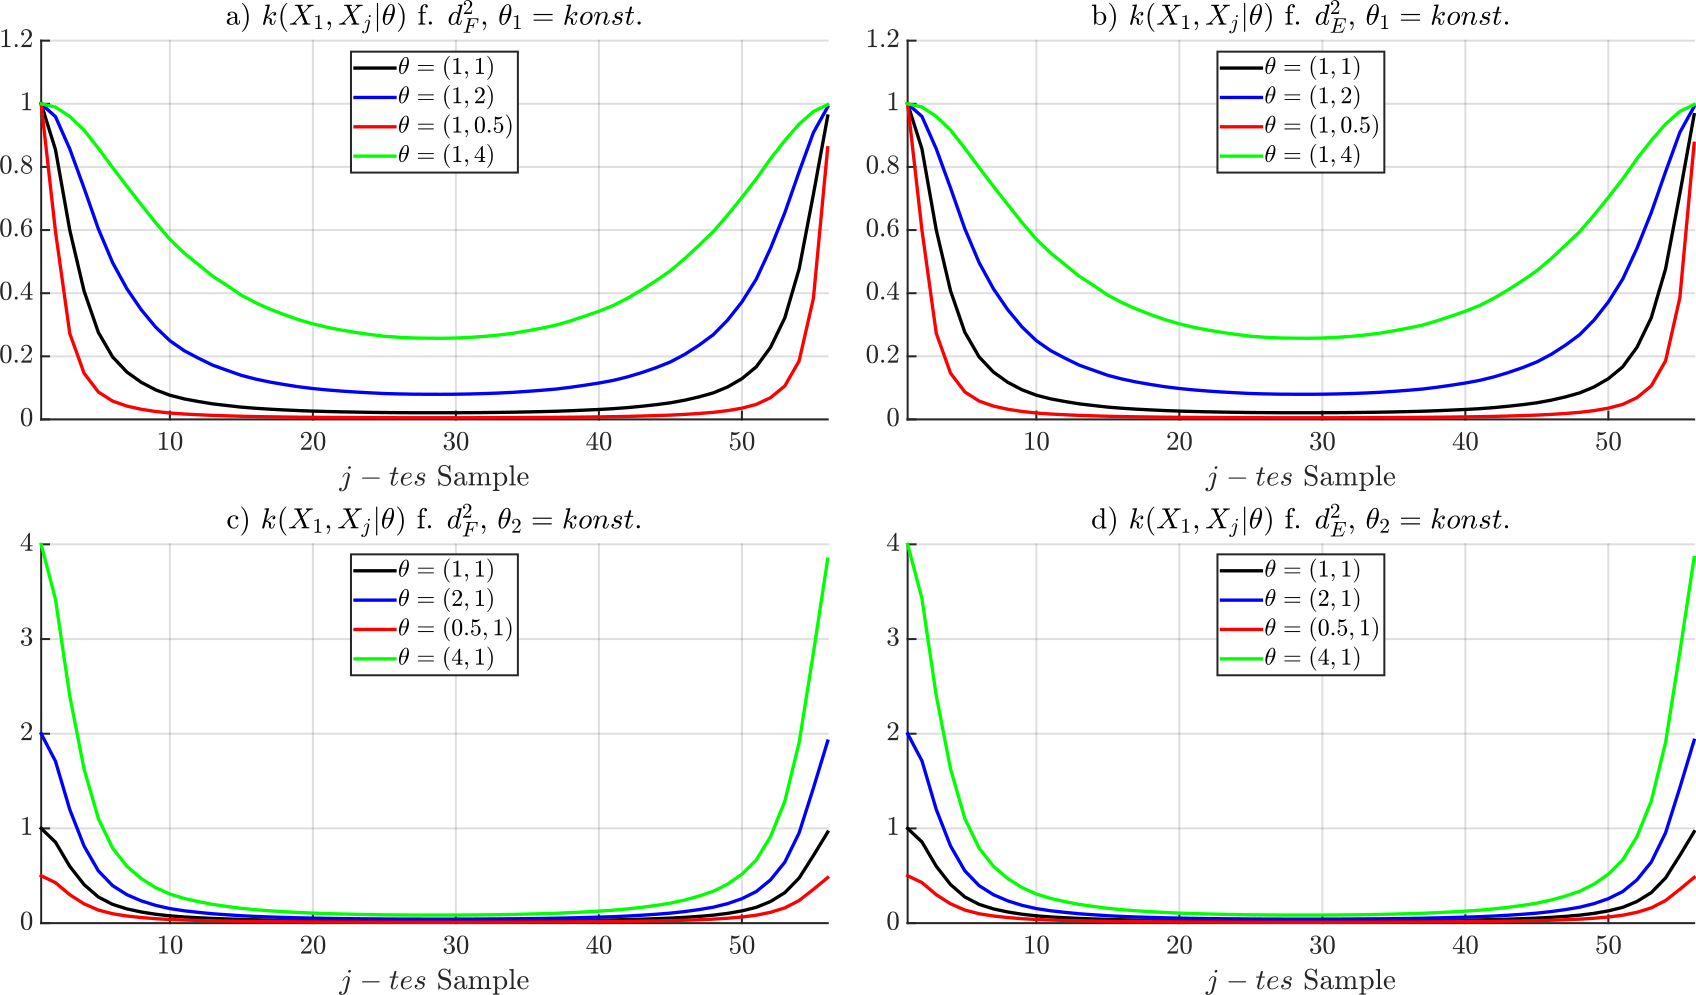
\includegraphics[width=\linewidth]{chapters/images/4-EuOExp/Vergleich-Kovarianzfunktionen}
\caption[Kovarianzfunktionen im Vergleich]{Kovarianzfunktionen im Vergleich für variierende Kernel-Parameter $\theta = (\sigma_f^2, \sigma_l)$ und $N_{Ref} = 56$ Referenzwinkel. Die Kovarianzfunktionen nach \autoref{eq:kfun} mit Frobenius-Norm nach \autoref{eq:df2} als Abstandsfunktion in den Abbildungen a) bzw. c) und mit euklidischer Norm nach \autoref{eq:de2innorm} in den Abbildungen b) bzw. d). Die Abbildungen a) und b) zeigen beide Funktionen mit variabler Längenskalierung $\theta_2 = \sigma_l$ und ausgeschalteter Höhenskalierung mit $\theta_1 = \sigma_f^2 = 1$. Vice versa sind beide Funktionen in den Abbildungen c) und d) gezeigt. Trainingsdaten basieren in a) und c) auf Matrizen. In b) und d) basieren Trainingsdaten auf Vektoren bzw. Skalare. Grafik nachempfunden aus \cite{Lang2014}.}
\label{fig:vergleich-kovarianzfunktionen}
\end{figure}


\clearpage
\begin{figure}[tph]
\centering
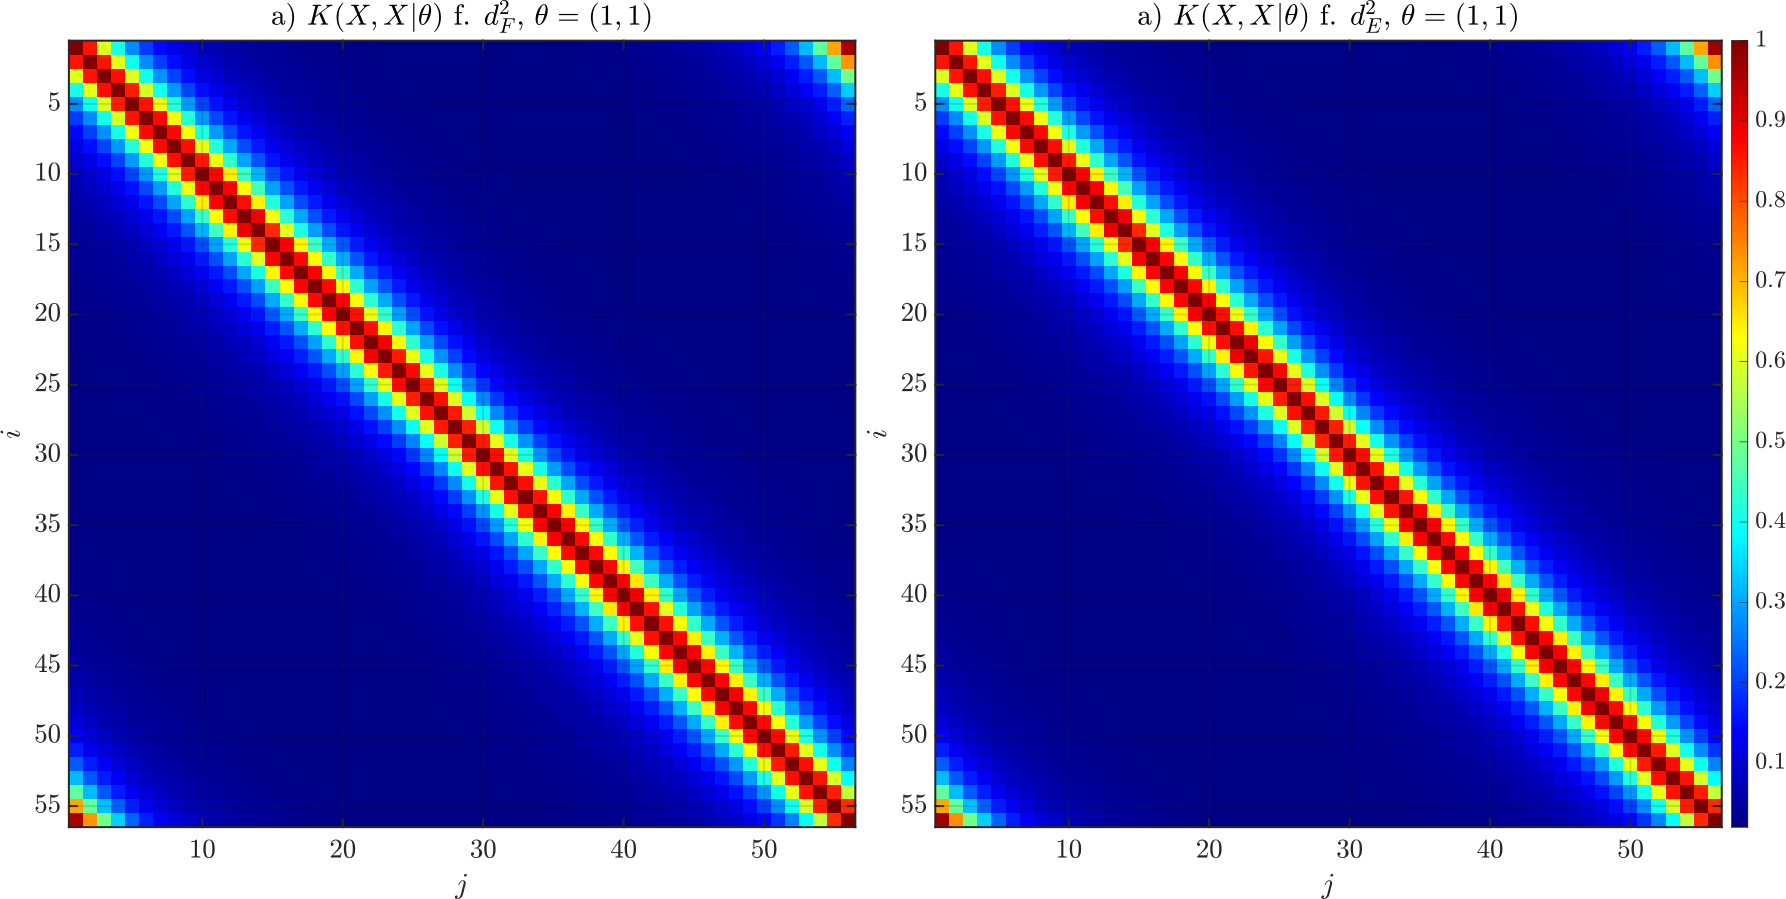
\includegraphics[width=\linewidth]{chapters/images/4-EuOExp/Vergleich-Kovarianzmatrizen}
\caption[Gegenüberstellung der Kovarianzmatrizen]{Gegenüberstellung der Kovarianzmatrizen bei ausgeschalteter Längen- und Höhenskalierung mit $\theta = (1,1)$ und $N_{Ref} = 56$ Referenzwinkel. In Abbildung a) nach Kovarianzfunktion mit Frobenius-Norm als Abstandsfunktion und in Abbildung b) mit euklidischen Abstand, siehe \autoref{eq:kfun}. In a) basieren Trainingsdaten auf Matrizen in b) auf Vektoren bzw. Skalare.}
\label{fig:vergleich-kovarianzmatrizen}
\end{figure}


\clearpage
\begin{figure}[tph]
\centering
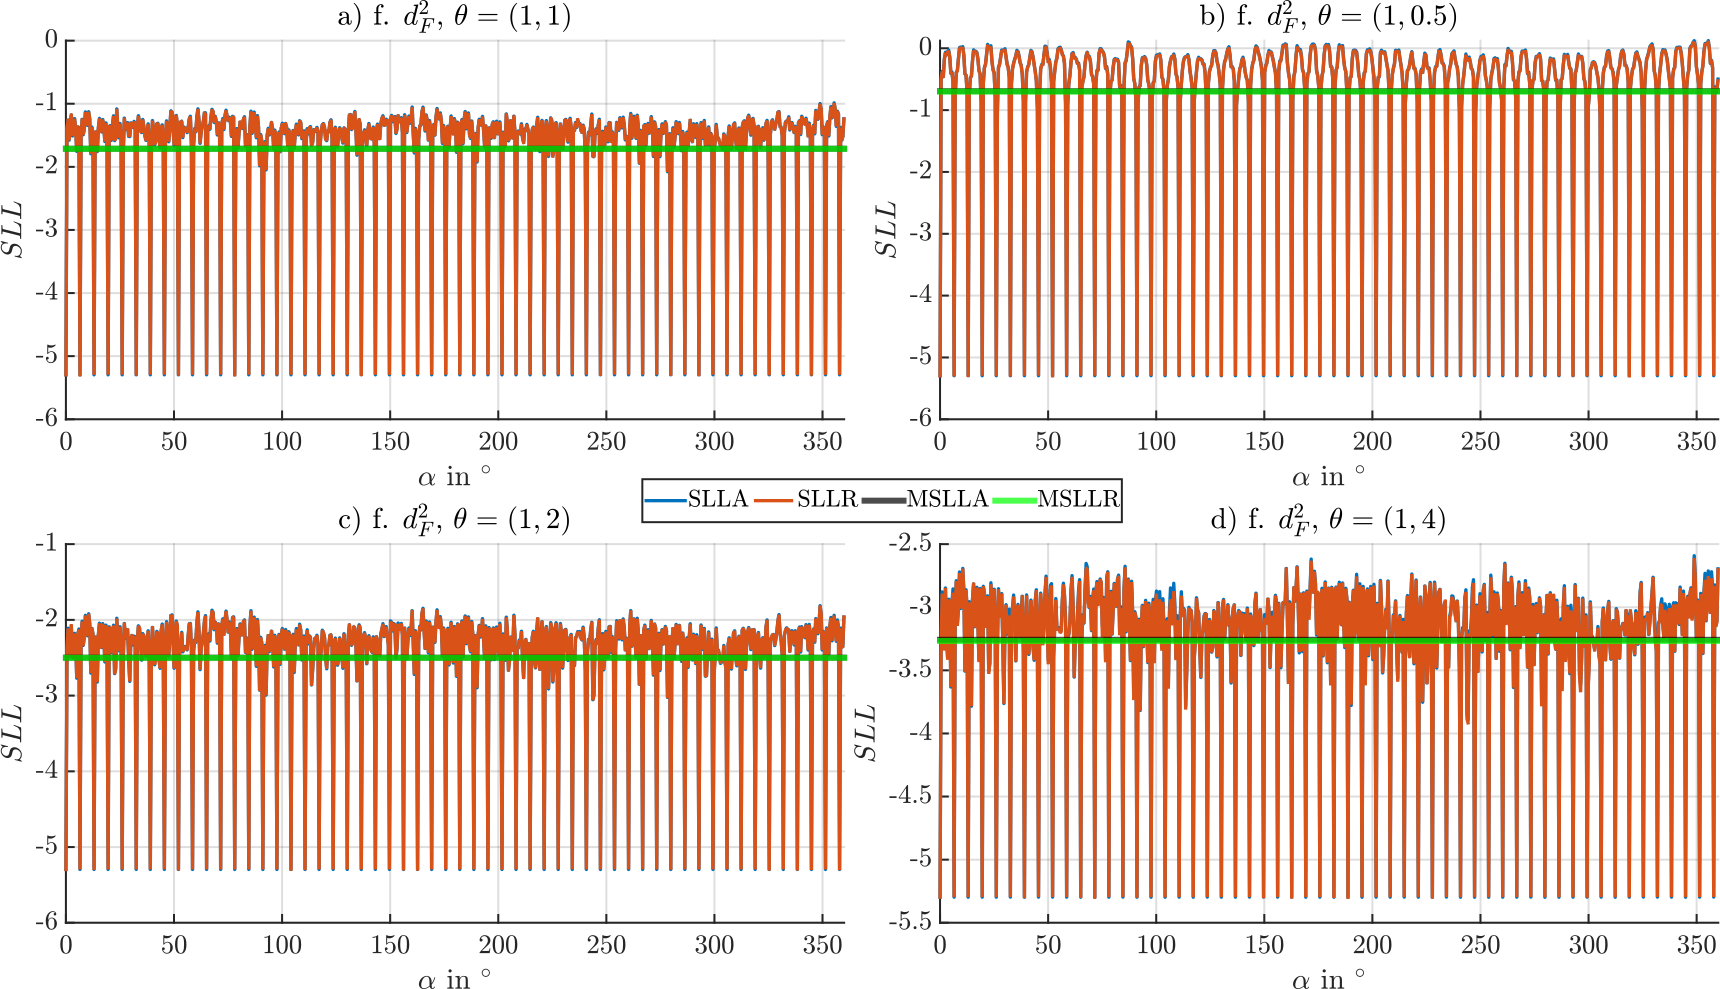
\includegraphics[width=\linewidth]{chapters/images/4-EuOExp/Vergleich-QFC-SLL}
\caption[Modellgeneralisierung mit Frobenius-Norm als Abstandfunktion]{Modellgeneralisierung mit Frobenius-Norm als Abstandfunktion nach \autoref{eq:kfun} und Trainingsdaten basierend auf Matrizen für $N_{Ref} = 56$ Referenzwinkel. Die Berechnungen zur Modellgeneralisierung erfolgten mit einem Testdatensatz für eine volle Rotation des Gebermagneten mit $720$ gleichverteilten Simulationswinkeln bei einer Winkelauflösung von $\SI{0,5}{\degree}$. Die Position des Sensors und die Magnetverkippung sind in beiden Datensätzen identisch. Variiert wurde die Längenskalierung $\theta_2 = \sigma_l$ bei ausgeschalteter Höhenskalierung $\theta_1 = \sigma_f^2 = 1$ der Kovarianzfunktion. Die Modellgeneralisierung wird über den standardisierten logarithmischen Verlust (engl. Loss) $SLL$ a. u. des Modells bewertet \cite{Rasmussen2006}. In Bezug auf Winkel (engl. Angle) mit $SLLA$ und Radius $SLLR$. Als Schwellwertkriterium dient die Mittlung (engl. Mean) der beiden Verluste zu $MSLLA$ und $MSLLR$ nach \autoref{eq:bayesopt}. Das Rauschniveau ist konstant mit $\sigma_n^2 = 10^{-6}$.}
\label{fig:vergleich-qfc-sll}
\end{figure}


\clearpage
\begin{figure}[tph]
\centering
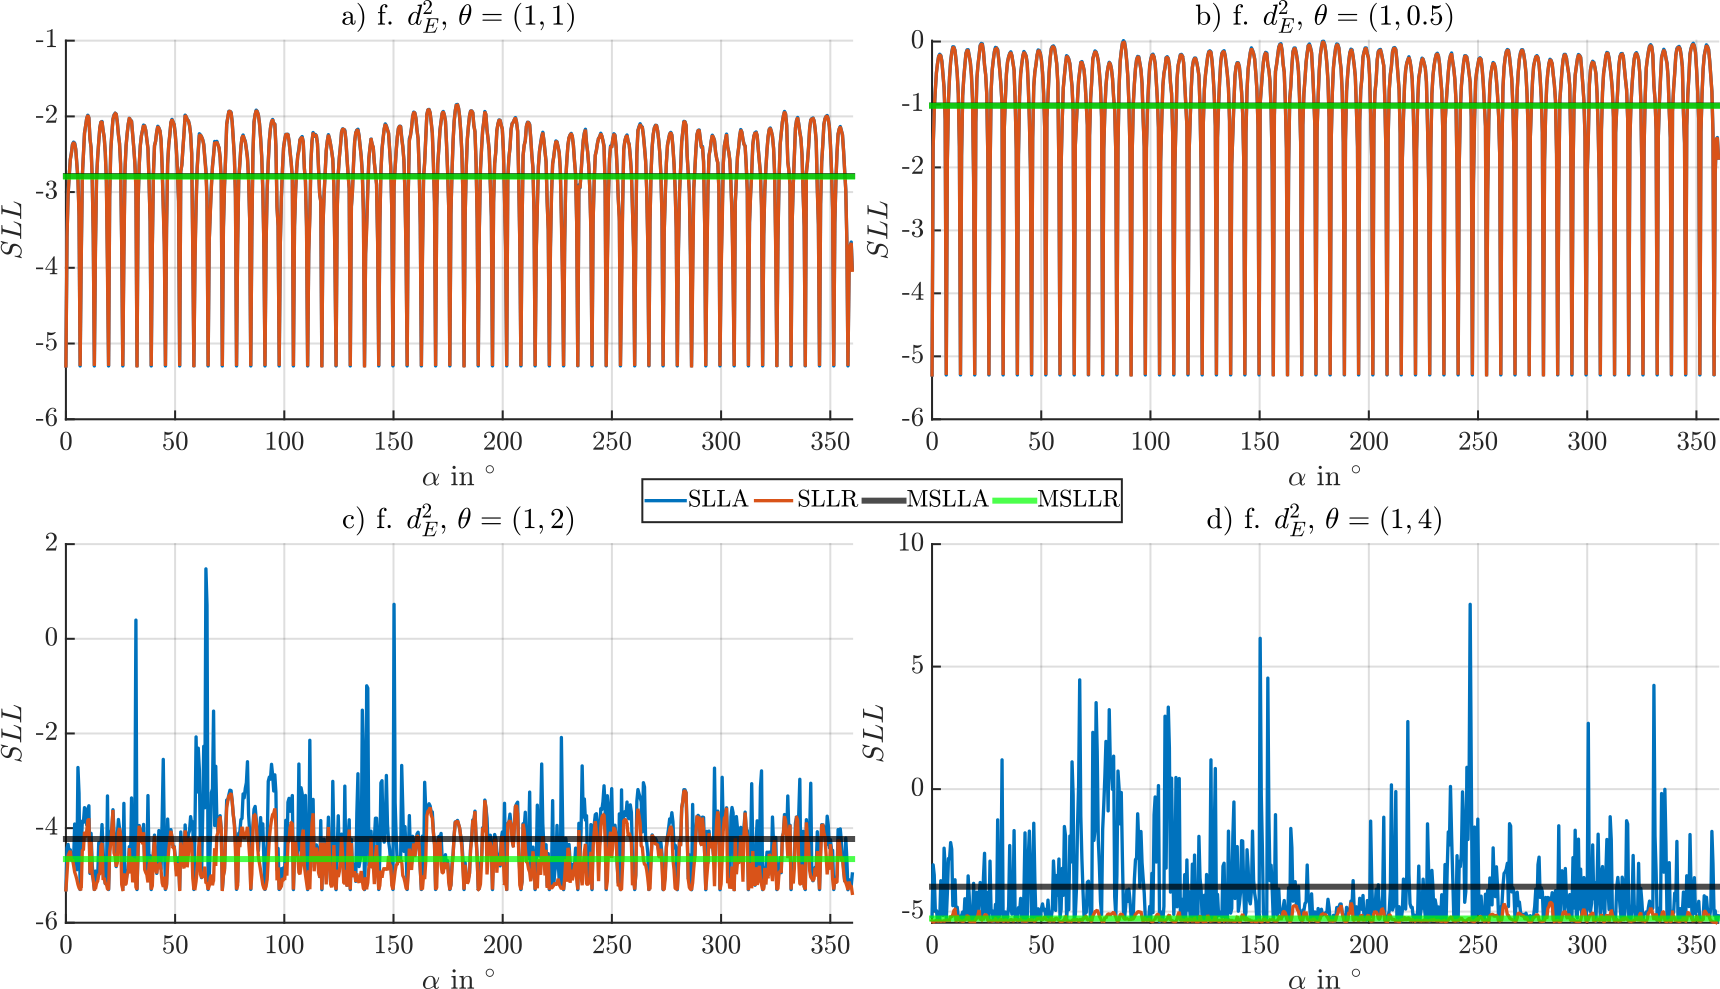
\includegraphics[width=\linewidth]{chapters/images/4-EuOExp/Vergleich-QFCAPX-SLL}
\caption[Modellgeneralisierung mit euklidischer Abstandsfunktion]{Modellgeneralisierung mit euklidischer Abstandsfunktion nach \autoref{eq:kfun} und Trainingsdaten basierend auf Vektoren bzw. Skalare für $N_{Ref} = 56$ Referenzwinkel. Die Berechnungen zur Modellgeneralisierung erfolgten mit einem Testdatensatz für eine volle Rotation des Gebermagneten mit $720$ gleichverteilten Simulationswinkeln bei einer Winkelauflösung von $\SI{0,5}{\degree}$. Die Position des Sensors und die Magnetverkippung sind in beiden Datensätzen identisch. Variiert wurde die Längenskalierung $\theta_2 = \sigma_l$ bei ausgeschalteter Höhenskalierung $\theta_1 = \sigma_f^2 = 1$ der Kovarianzfunktion. Die Modellgeneralisierung wird über den standardisierten logarithmischen Verlust (engl. Loss) $SLL$ a. u. des Modells bewertet \cite{Rasmussen2006}. In Bezug auf Winkel (engl. Angle) mit $SLLA$ und Radius $SLLR$. Als Schwellwertkriterium dient die Mittlung (engl. Mean) der beiden Verluste zu $MSLLA$ und $MSLLR$ nach \autoref{eq:bayesopt}. Das Rauschniveau ist konstant mit $\sigma_n^2 = 10^{-6}$.}
\label{fig:vergleich-qfcapx-sll}
\end{figure}
\clearpage


% !TEX root = ../thesis.tex
% adjust number of reference angles
% @author Tobias Wulf
%

\section{Anpassung der Referenzwinkelanzahl}\label{sec:exp2}


\textbf{Zweck:} Das Experiment soll einen Bereich abstecken für die Wahl der Anzahl für gleichverteilte Referenzwinkel. Dafür wird die äußere Modelloptimierung über das Rauschniveau nach \autoref{alg:bayesopt} ausgeschaltet und ein konstantes Rauschniveau $\sigma_n^2$ vorgeben. Das Regressionsmodell wird daher nur für die Längen- und Höhenskalierung $\theta = (\sigma_f^2, \sigma_l)$ der Kovarianzfunktion optimiert, siehe \autoref{alg:fminconopt}. Verglichen wird das Regressionsmodell für euklidischen Abstand nach \autoref{eq:de2innorm} und \autoref{eq:kfun} einmal ohne unterstützende Mittelwertbildung über Polynome (Zero-Mean) und mit Polynombildung ersten Grades, siehe \autoref{eq:hfun} bis \autoref{eq:gprmean}. Diese wirkt als eine Offset- und Amplitudenkorrektur der Messwerten. Es werden absolute mittlere und maximale Winkelfehler in Abhängigkeit der Referenzwinkelanzahl verglichen. Zusätzliche wird die Berechnungsdauer einer Winkelvorhersage in Abhängigkeit der Referenzwinkelanzahl bzw. Trainingspunkte aufgenommen. Im besten Fall stellt sich heraus, dass das Mittelwert freie Verfahren gleich oder besser ist gegenüber dem Polynom gestützten Verfahren. Die Umsetzung des letzteren Verfahrens ist deutlich aufwendiger zu gestalten und birgt einige numerischer Fehleranfälligkeiten und Hürden, die es in den Griff zu bekommen gilt.

\textbf{Durchführung:} Es werden zwei Modelle mit euklidischer Abstandfunktion initialisiert und Trainiert, jeweils mit und ohne unterstützendes Mittelwertpolynom. Jedes der beiden Modelle wird mit pro Durchgang mit gleichem Trainingsdaten trainiert und anschließend die Skalierung der Kovarianzfunktion in Länge und Höhe entsprechend der Trainingsdaten getrimmt. Danach wird die Zeit gemessen, die es benötigt einen Simulationswinkel zu vorherzusagen. Jeweils getrennt für beide Modelle. Zum Ende des Durchgangs werden absolute Winkelfehler auf eine volle Rotation mit einem Testdatensatz über $720$ Winkeln bei einer Auflösung von $\SI{0,5}{\degree}$ berechnet und für mittlere sowie maximale Winkelfehler über die gesamte Rotation ausgewertet. Ebenfalls für beide Modelle. Der Durchgang wird für jeden zur Verfügung stehenden Trainingsdatensatz wiederholt. Der Testdatensatz bleibt für jeden Durchgang gleich. Alle Datensätze sind für die gleiche Position des Sensors und bei gleicher Verkippung des Magneten zuvor prozessiert worden.

\textbf{Erzeugte Datensätze:} Es sind für das Experiment 12 Trainingsdatensätze mit unterschiedlicher Referenzwinkelanzahl und ein Testdatensatz erzeugt worden. Alle Datensätze korrespondieren in Position und Verkippung.

\textbf{Matlab-Skript:} compareCpuTimeVsError.m, siehe \autoref{mcode:comparecputimevserror}.


\clearpage


\textbf{Abweichende Parameter von \autoref{tab:sim-params-exp}:}

\begin{itemize}
	\item TrainingsOptions: nAngles: $\left\{ 8, 16, 24, 32, 40, 48, 60, 80, 120, 240, 360, 720 \right\}$
	\item GRPOptions: kernel : 'QFCAPX'
	\item GPROptions: mean: 
	\begin{itemize}
		\item[a.] 'zero'
		\item[b.] 'poly'
	\end{itemize}
\end{itemize}

\textbf{Ergebnisse:} Die Ergebnisse des Experiments sind grafisch in \autoref{fig:timings-vs-errors} ausgewertet. Berechnungszeiten für einen Simulationswinkel a) sowie mittlerer b) und maximaler c) absoluter Winkelfehler bei voller Rotation sind in Abhängigkeit der Referenzwinkelanzahl in den Trainingsdatensätzen aufgetragen.

\textbf{Beobachtungen:} Die Messung der Berechnungszeit für eine Simulationswinkelvorhersage in a) ergibt, dass beide Implementierungskonfigurationen annähernd gleich schnell sind und die Rechenzeit bis eine Referenzwinkelanzahl von $N_{Ref} = 80$ mit leichten Abweichungen konstant bleibt. Für eine Referenzwinkelanzahl von $N_{Ref} > 80$ nimmt die Rechenzeit für beide Varianten gleichermaßen exponentiell zu. Für absolute mittlere und maximale Winkelfehler unterscheiden sich die mittelwertfreie und Polynom gestützte Variante nur bei $N_{ref} = 8$. Dort liefert jeweils die mittelwertfreie Variante den geringeren Winkelfehler. Für eine Referenzwinkelanzahl $N_{Ref} > 8$ liefern beide Variationen einen annähernd gleichen Winkelfehler. Bei einer Referenzwinkelanzahl von $N_{Ref} = 48$ gibt es eine Sprungstelle für den mittleren und maximalen Winkelfehler, beide mittlerer sowie maximaler Winkelfehler verringern sich ungefähr um die Hälfte. Der Winkelfehler bleibt nach dem Sprung konstant und schwankt nur noch minimal. Dieser Bereich (2) ist in den Abbildungen b) und c) grau unterlegt und weißt im Vergleich zu Bereich (1) weniger Fehlerdynamik für nachfolgende Optimierungsschritte auf. Der interessante Bereich (1) für eine weitere Optimierung über das Rauschniveau $\sigma_n^2$ nach \autoref{alg:bayesopt} ist in a), b) und c) grün unterlegt. Diesen gilt es im weiteren Verlauf anzupassen und die Sprungstelle in b) und c) zu verkleinern oder auszulöschen.


\clearpage
\begin{landscape}
\begin{figure}[tbph]
	\centering
	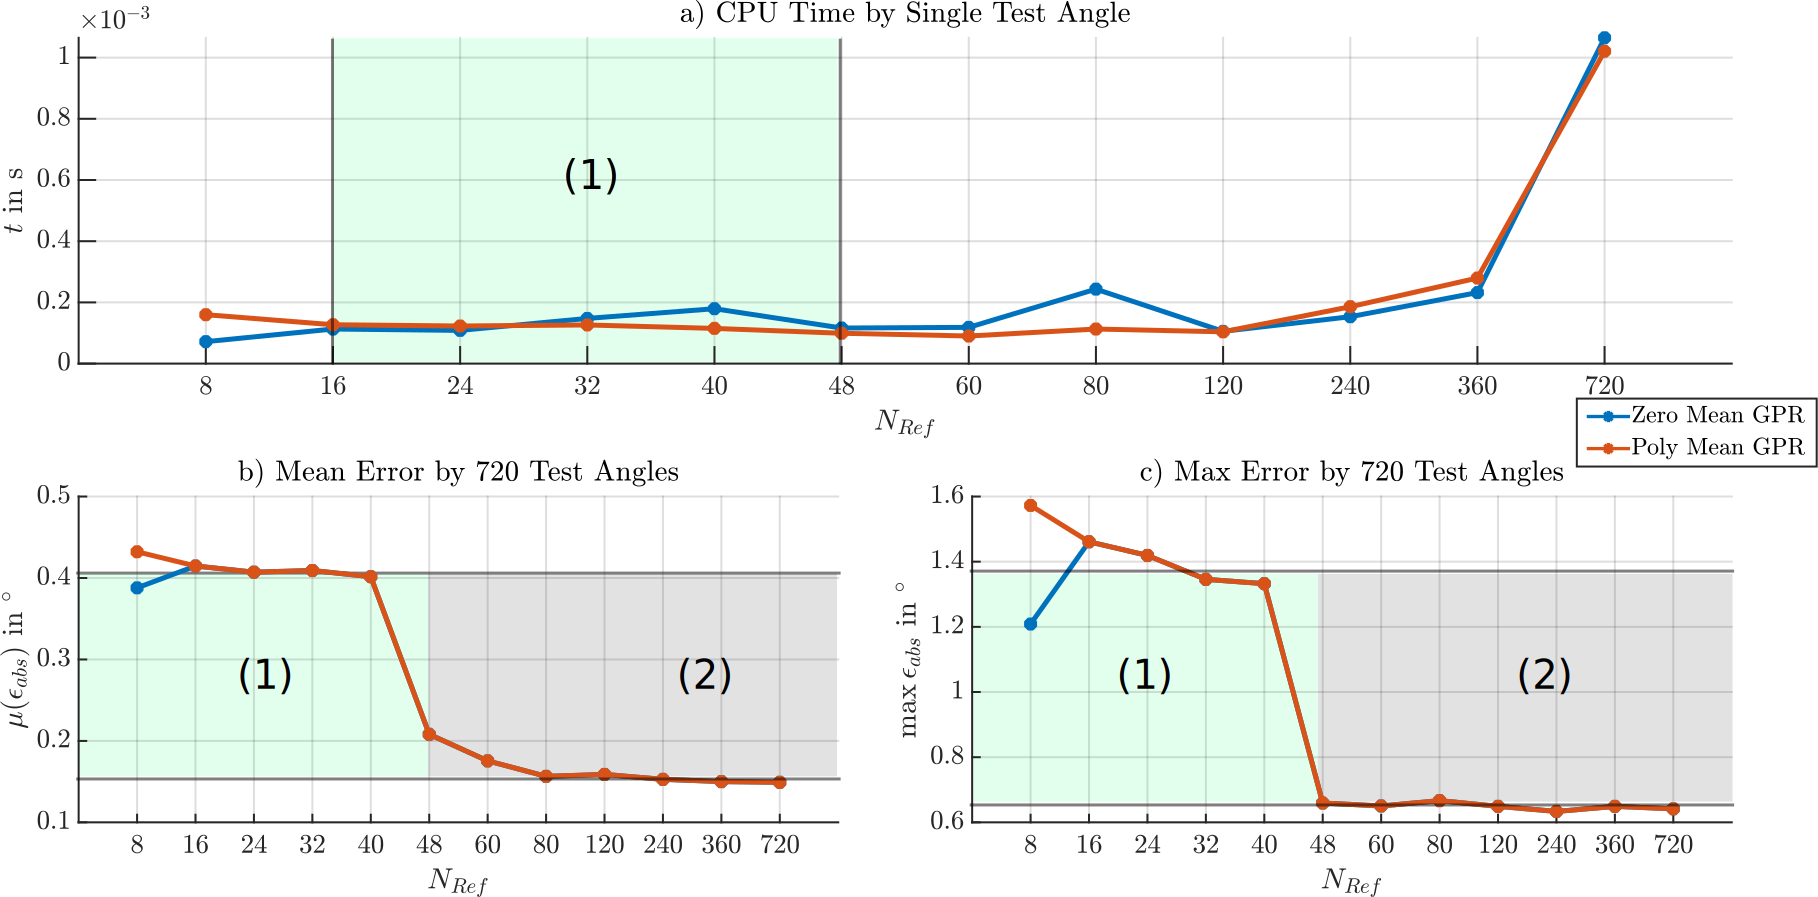
\includegraphics[width=\linewidth]{chapters/images/4-EuOExp/Timings-vs-Errors}
	\caption[Variation der Referenzwinkelanzahl bei konstantem Rauschniveau]{Variation der Referenzwinkelanzahl bei konstantem Rauschniveau $\sigma_n^2 = 10^{-6}$. Es wird die Implementierung des Regressionsmodell nach \autoref{eq:kfun} mit euklidischen Abstand nach \autoref{eq:de2innorm}, jeweils ohne (Zero Mean GPR) und mit Mittelwertunterstützung (Poly Mean GPR) in Abhängigkeit der Referenzwinkelanzahl $N_{Ref}$ verglichen. Dafür wird in a) die Berechnungszeit eines Simulationswinkel gemessen und in b) der absolute mittlere Winkelfehler, sowie in c) der absolute maximale Winkelfehler auf eine volle Rotation ausgewertet. Die jeweiligen initiierten Modellvariation sind für ihre Kovarianzfunktionsparameter $\theta = (\sigma_f^2,\sigma_l)$ getrimmt nach \autoref{alg:fminconopt}. Die Optimierung des Rauschniveaus $\sigma_n^2$ nach \autoref{alg:bayesopt} ist ausgeschaltet. Modelltrainingsdaten basieren hier für beide Varianten auf Vektoren bzw. Skalare.}
	\label{fig:timings-vs-errors}
\end{figure}
\end{landscape}


\clearpage

	
% !TEX root = ../thesis.tex
% adjust noise level
% @author Tobias Wulf
%

\section{Anpassung des Rauschniveaus für Noisy-Observation}\label{sec:exp3}


\textbf{Zweck:} Das Experiment ist eine Fortsetzung zum \autoref{sec:exp2} und schaltet zusätzlich zur Trimmung der Kovarianzfunktion nach \autoref{alg:fminconopt} die äußere Modelloptimierung über das Rauschniveau $\sigma_n^2$ nach \autoref{alg:bayesopt} ein. Es dient primär zur weiteren Anpassung der Referenzwinkelanzahl und untersucht sekundär die Möglichkeit zur Winkelfehlerminimierung, unter Berücksichtigung der gemachten Beobachtungen im \autoref{sec:exp2}. Ziel ist es hier einen Kompromiss zu finden, bestehend aus brauchbarer Generalisierung und akzeptablen Winkelfehler bei möglichst geringer Referenzwinkelanzahl. Dafür werden für jeden Durchgang Modellverlust, absoluter mittlerer Winkelfehler sowie der maximale Winkelfehler auf eine volle Rotation mit $720$ Simulationswinkeln bei einer Auflösung von $\SI{0,5}{\degree}$ berechnet. Dafür wird wie in \autoref{sec:exp2} das Regressionsmodell für euklidischen Abstand nach \autoref{eq:de2innorm} und \autoref{eq:kfun} in beiden Varianten einmal als mittelwertfreies Modell und Mittelwert unterstütztes Modell betrieben. Es wird der in \autoref{fig:timings-vs-errors} grün gekennzeichnete Bereich (1) näher untersucht.

\textbf{Durchführung:} Die Durchführung ist aus \autoref{sec:exp2} zu entnehmen. Änderungen in der Durchführung beziehen sich auf die Ausführungen zur Ermittlung der Berechnungszeit für eine Winkelvorhersage, diese ist durch die Berechnung der Modellverluste für Winkel ersetzt.

\textbf{Erzeugte Datensätze:} Es sind für das Experiment 24 Trainingsdatensätze mit unterschiedlicher Referenzwinkelanzahl und ein Testdatensatz erzeugt worden. Alle Datensätze korrespondieren in Position und Verkippung.

\textbf{Matlab-Skript:} compareNoiseOptAbility.m, siehe \autoref{mcode:comparenoiseoptability}.

\textbf{Abweichende Parameter von \autoref{tab:sim-params-exp}:}

\begin{itemize}
	\item TrainingsOptions: nAngles: $\left\{ 8, 9, 10, \ldots, 29, 30, 31 \right\}$, inkrementiert um 1
	\item GRPOptions: kernel : 'QFCAPX'
	\item GPROptions: mean: 
	\begin{itemize}
		\item[a.] 'zero'
		\item[b.] 'poly'
	\end{itemize}
\end{itemize}


\clearpage


\textbf{Ergebnisse:} Die Ergebnisse des Experiments sind grafisch in \autoref{fig:msll-vs-errors} ausgewertet. Modellverlust für Winkel in a), sowie mittlerer b) und maximaler c) absoluter Winkelfehler. Alle drei durchgeführten Berechnungen erfolgten für jeden Durchgang mit voller Rotation um $720$ Testwinkel und sind in Abhängigkeit der Referenzwinkelanzahl in den Trainingsdatensätzen aufgetragen.

\textbf{Beobachtungen:} Die Betrachtung der Generalisierung in \autoref{fig:msll-vs-errors} a) über den mittleren standardisierten logarithmischen Verlust $MSLL$ (hier für Winkelverluste) zeigen, dass bei zunehmender Referenzwinkelanzahl $N_{Ref}$ sich die Generalisierung verbessert und das Regressionsmodell besser auf von den Trainingsdaten abweichende Datensätze reagiert. Auftretende Schwankungen in der Generalisierung a) bilden sich gleichermaßen in den Winkelfehlern b) und c) ab. In Bezug auf die gemachten Beobachtungen aus \autoref{sec:exp2} und \autoref{fig:timings-vs-errors} Bereich (1) ist es gelungen den mittleren und maximalen Winkel weiter zu drücken. Der mittlere Winkelfehler in b) und maximale Winkelfehler in c) schwingen sich der Generalisierung folgend auf die Winkelfehlerniveaus aus \autoref{fig:timings-vs-errors} b) und c) ein. Ein möglicher Kompromiss aus Generalisierung, Winkelfehler und möglichst geringer Referenzwinkelanzahl ist für $N_{Ref} = 17$ in \autoref{fig:msll-vs-errors} markiert.


\clearpage
\begin{landscape}
\begin{figure}[tbph]
	\centering
	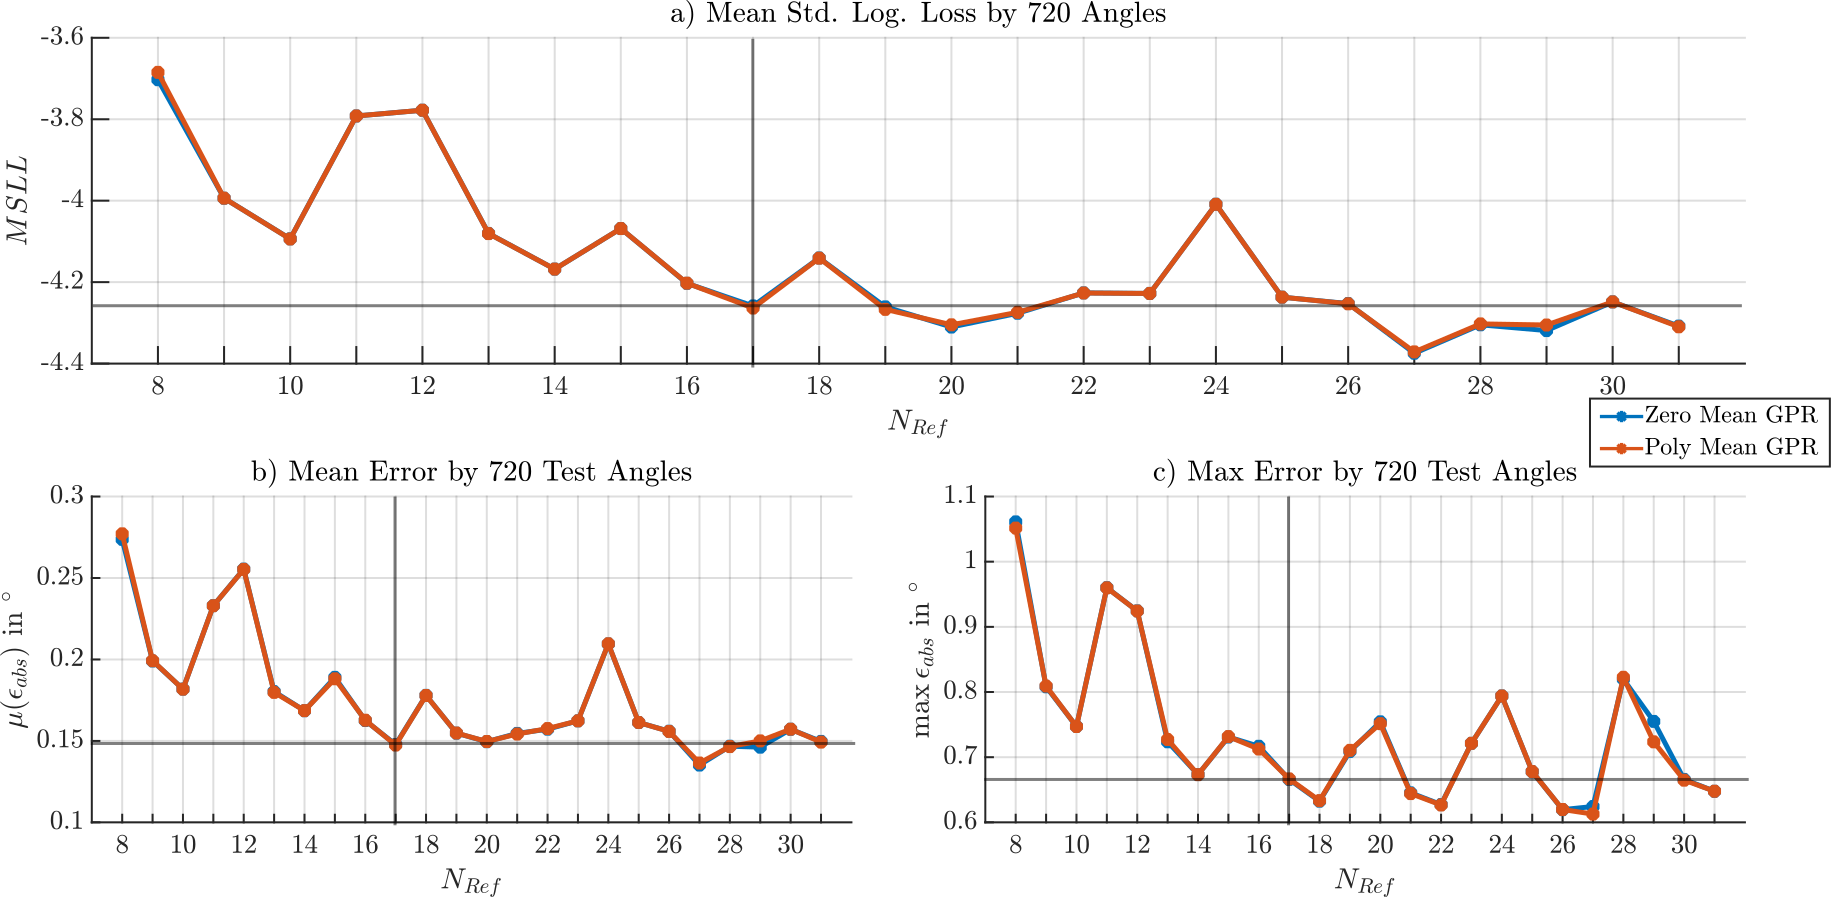
\includegraphics[width=\linewidth]{chapters/images/4-EuOExp/MSLL-vs-Errors}
	\caption[Variation der Referenzwinkelanzahl mit Optimierung des Rauschniveau]{Variation der Referenzwinkelanzahl mit Optimierung des Rauschniveaus $\sigma_n^2$ nach \autoref{alg:bayesopt}. Es wird die Implementierung des Regressionsmodell nach \autoref{eq:kfun} mit euklidischen Abstand nach \autoref{eq:de2innorm}, jeweils ohne (Zero Mean GPR) und mit Mittelwertunterstützung (Poly Mean GPR) in Abhängigkeit der Referenzwinkelanzahl $N_{Ref}$ verglichen. Dafür wird in a) die Modellgeneralisierung über den mittleren standardisierten logarithmischen Verlust (engl. Loss) $MSLL$ a. u. nach \autoref{eq:bayesopt} bewertet. Die Verlustberechnung ist für Winkelverluste konfiguriert. In b) folgen der absolute mittlere Winkelfehler, sowie in c) der absolute maximale Winkelfehler. Alle drei Berechnungen sind jeweils für jeden Schritt auf eine volle Rotation durchgeführt worden. Modelltrainingsdaten basieren hier auf Vektoren bzw. Skalare.}
	\label{fig:msll-vs-errors}
\end{figure}
\end{landscape}


\clearpage


% !TEX root = ../thesis.tex
% adjust parameter limits
% @author Tobias Wulf
%

\section{Anpassung der Parametergrenzen}\label{sec:exp4}

\textbf{Zweck:}

\textbf{Durchführung:}

\textbf{Erzeugte Datensätze:}

\textbf{Matlab-Skript:}

\textbf{Abweichende Parameter von \autoref{tab:sim-params-exp}:}

Abweichende Parameter:

\begin{itemize}
	\item TrainingsOptions: nAngles: 17
	\item GRPOptions: kernel : 'QFCAPX'
	\item $\sigma_f^2$-Bounds: $(1,10)$
	\item $\sigma_l$-Bounds: $(10,30)$
	\item $\sigma_n^2$-Bounds: $(10^{-6},10^{-4})$
	\item GPROptions: mean: 'zero'
	\item OptimRuns 10
\end{itemize}


\textbf{Ergebnisse:}

Anpassung:

$\sigma_f^2$-Bounds: $(1, 10)$ / $\sigma_l$-Bounds: $(10, 30)$ / $\sigma_n^2$-Bounds: $(10^{-6}, 10^{-4})$
Anpassung: Durchlaufzahl 10

\textbf{Beobachtungen:}


\clearpage
\begin{landscape}
\begin{figure}[tbph]
	\centering
	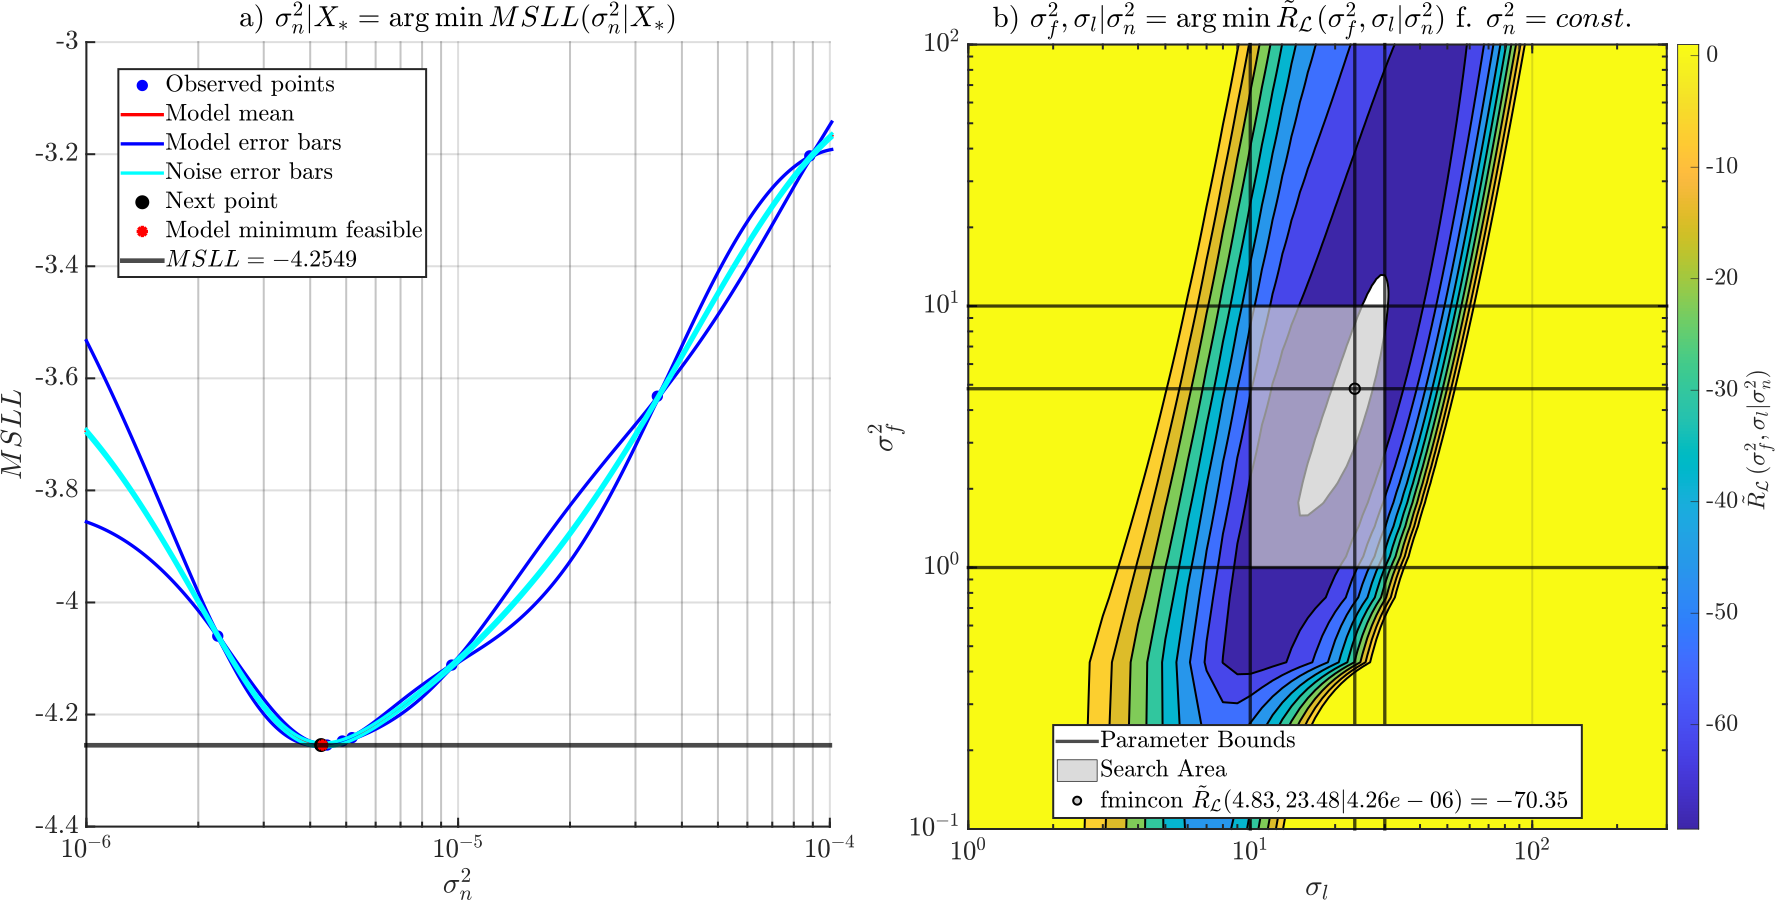
\includegraphics[width=\linewidth]{chapters/images/4-EuOExp/QFCAPX-Z-N17-Bounds}
	\caption[Angepaster Parameter Bounds]{Angepaster Parameter Bounds}
	\label{fig:qfcapx-z-n17-bounds}
\end{figure}
\end{landscape}


\clearpage
\begin{landscape}
\begin{figure}[tbph]
	\centering
	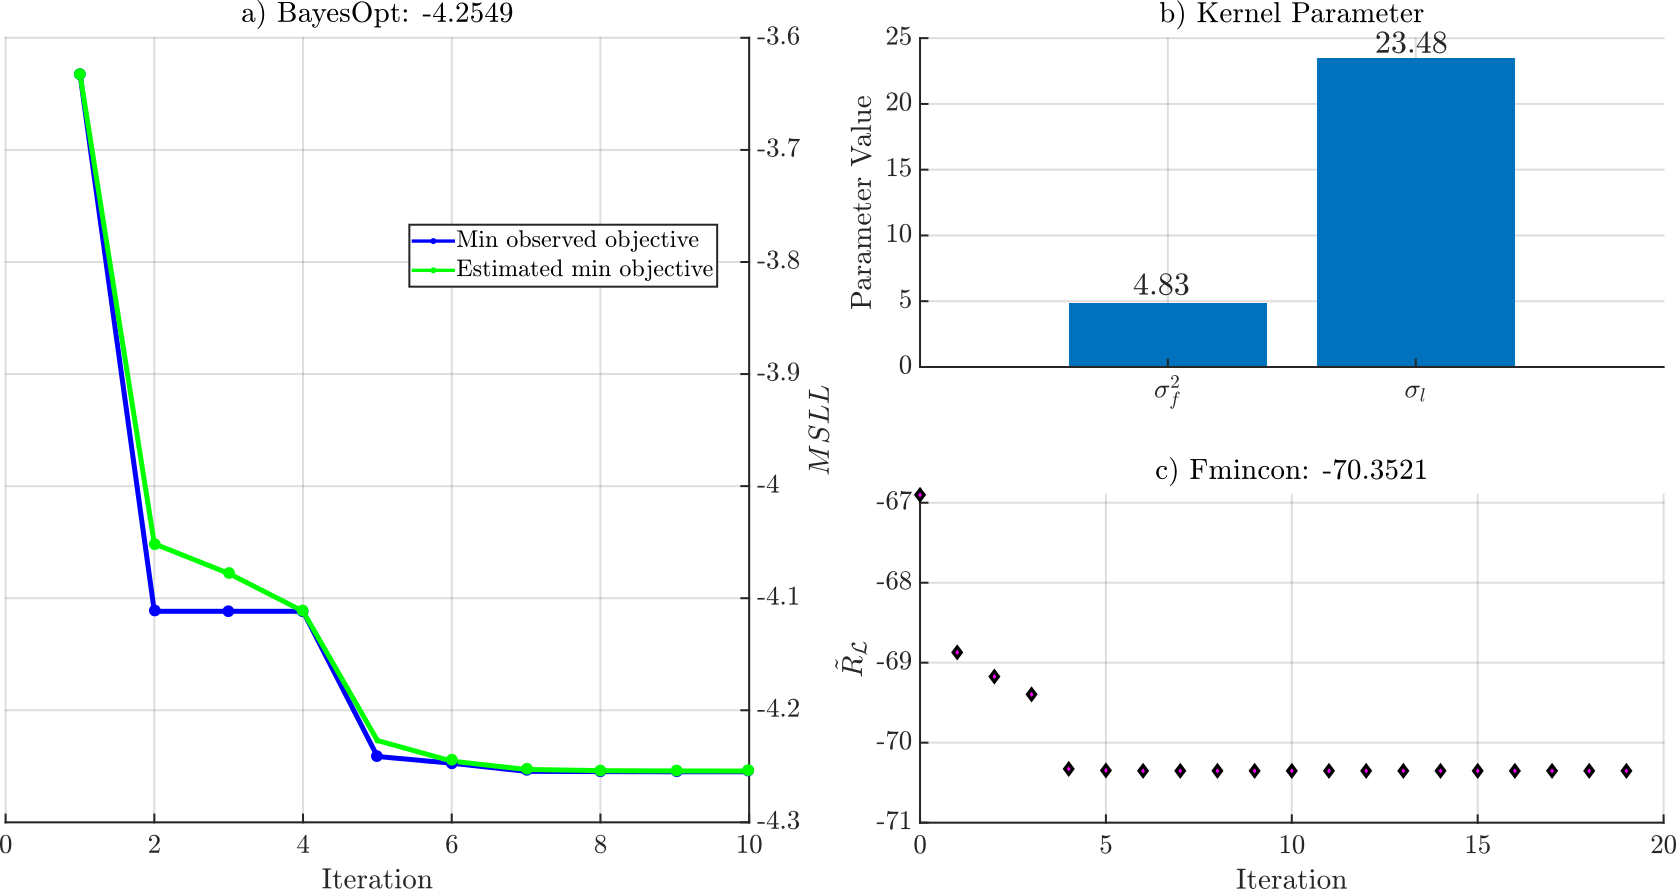
\includegraphics[width=\linewidth]{chapters/images/4-EuOExp/QFCAPX-Z-N17-Opt}
	\caption[QFCAPX Z N17 Optimierung Runs 10]{QFCAPX Z N17 Optimierung Runs 10}
	\label{fig:qfcapx-z-n17-opt}
\end{figure}
\end{landscape}


\clearpage


% !TEX root = ../thesis.tex
% behavior at simple misalignments
% @author Tobias Wulf
%

\section{Verhalten bei einfachen Fehllagen}\label{sec:exp5}

\textbf{Zweck:} Das Experiment ist als Stichprobenexperiment für räumliche Fehllagen des Sensors und Verkippungen des Magneten zu betrachten und soll erste Einschätzungen des Verhalten bei einfachen Fehllagen liefern. Für eine vollständige Charakterisierung des Sensormodells muss in einem abgesteckten räumlichen Bereich jede Position mit jeder möglichen Verkippung angefahren werden. Dieses würde allerdings den Rahmen dieser Arbeit weit überschreiten und muss gesondert in nachfolgenden Arbeiten durchgeführt werden. Das Experiment ist wird mit $N_{Ref} = 17$ Referenzwinkeln für das Regressionsmodell nach mit euklidischer Abstandsfunktion nach \autoref{eq:de2innorm} und resultierender Kovarianzfunktion nach \autoref{eq:kfun} durchgeführt. Das Modell wird als mittwertfreier Kernel betrieben.

\textbf{Durchführung:} Zum Beginn des Experiments werden Drift Parameter für die räumlichen Verschiebungen des Sensors und der Verkippung des Magnet gesetzt. Basierend darauf werden im Anschluss alle notwendigen Datensätze automatisch generiert und indiziert. Es wird eine Referenzposition bei $(0;0;7,5)^T$ mm unter dem Magneten und $\SI{0}{\degree}$ Magnetverkippung festgelegt. Auf dieser Position wird ein Referenzmodell einmalig trainiert. Beginnend mit der Verschiebung in $X$ wird jeder Drift sequentiell hintereinander ausgeführt. Es folgen Drift in $Y$ und $Z$, sowie abschließend die Verkippung des Magneten. In $X$ $Y$ und $Z$ wird der Sensor jeweils um $\pm 3$ mm in $0,25$ mm Schritten relativ zur Referenzposition versetzt. Für den Drift in $Z$ deckt das ungefähr den Bereich von Sättigung bis Kennfeldmittelpunkt des TMR-Sensor-Kennfeldes ab, siehe \autoref{ch:tdk-datensatz}. Die Verkippung des Magneten wird von $\SI{0}{\degree}$ bis $\SI{12}{\degree}$ in $\SI{0,5}{\degree}$ Schritten vorgenommen. Bei jeder Driftposition wird eine volle Rotation mit $720$ Simulationswinkel bei einer Auflösung von $\SI{0,5}{\degree}$ durchgeführt. Es werden absolute Winkelfehler des Referenzmodells für den mittleren und maximalen Fehler auf die volle Rotation ausgewertet. Zusätzlich zum Referenzmodell wird ein zweites Modell mit gleich Konfiguration initialisiert. Dieses wird bei jedem Drift auf die aktuelle Position trainiert, was ein erneutes Trainieren des Referenzmodells simulieren soll. Für das zweite Modell werden ebenfalls mittlerer und maximaler Winkelfehler erfasst, sowie die Modellparameter $\sigma_f^2$, $\sigma_l$ und das Rauschniveau $\sigma_n^2$. Im Vergleich zu \autoref{sec:exp4} sind hier die Parametergrenzen geweitet und die Durchlaufzahl der Optimierung erhöht, um den Algorithmen genügend Reserve zur Verfügung zu stellen und das Verletzen von Parametergrenzen zu verhindern. Der Simulation nachfolgend werden Best- und Worst-Case Positionen des Experiments separat simuliert und im detaillierter Dargestellt.


\clearpage


\textbf{Erzeugte Datensätze:} Jeweils 100 Trainings- und Testdatensätze mit korrespondierenden Positionen des Sensors und Verkippungswinkel des Magneten. Die Datensätze werden zum Beginn des Experiments entsprechend der Driftvorgaben prozessiert, indiziert und zur Driftausführung geladen.

\textbf{Matlab-Skript:} compareMissAlign.m und demoGPRModule.m, siehe \autoref{mcode:comparemissalign} und \autoref{mcode:demogprmodule}.

\textbf{Abweichende Parameter von \autoref{tab:sim-params-exp}:}

\begin{itemize}
	\item TrainingsOptions: nAngles: 17
	\item TrainingsOptions/ TestOptions: xPos/ yPos: $-3:0,25:3$
	\item TrainingsOptions/ TestOptions: zPos: $4,5:0,25:10,5$
	\item TrainingsOptions/ TestOptions: tilt: $0:0,5:12$
	\item GRPOptions: kernel : 'QFCAPX'
	\item $\sigma_f^2$-Bounds: $(0.1,100)$
	\item $\sigma_l$-Bounds: $(1,100)$
	\item $\sigma_n^2$-Bounds: $(10^{-7},10^{-3})$
	\item GPROptions: mean: 'zero'
	\item OptimRuns 30
\end{itemize}

\textbf{Ergebnisse:} Die Ergebnisse der Simulation sind grafisch ausgewertet. In \autoref{fig:drift-model-errors} sind die Winkelfehler in Bezug auf Verschiebung des Sensors und Verkippung des Magneten erfasst.
\autoref{fig:drift-horizontal-model-parms} und \autoref{fig:drift-vertical-model-parms} zeigen, die während des Experiments festgehalten Modellparameter bei horizontalen und vertikalen Drift sowie Verkippung. In \autoref{fig:z-pos-comp-45-105-rotation} ist der Best-Case bei Drift in $z = 0,45$ mm und der Worst-Case bei Drift in $z = 10,5$ mm gesondert nebeneinander dargestellt.


\clearpage


\textbf{Beobachtungen:} Der Drift des Referenzmodell zeigt in \autoref{fig:drift-model-errors}, dass das Sensormodell sensibler auf vertikalen als auf horizontalen Versatz reagiert. Für die horizontale Verschiebung in $X$ und $Y$ zeichnet sich ein Pufferbereich von $\pm 0,5$ mm ab. Eine entsprechende Reaktion auf vertikalen Versatz in $Z$ zeigt schon bei $\pm 0,25$ mm vor. Die Winkelfehler nehmen dann exponentiell bei Vergrößerung des Versatzes zu. Im $Z$-Drift von $6,25$ mm bis $4,5$ mm stagniert der mittlere Winkelfehler. Im $X$-Drift ab $\pm 2,75$ mm kommt es zu Intervallüberschreitungen in der $\textrm{atan2}$-Funktion bei der Winkelrückrechnung, zu sehen am sprunghaften Anstieg des maximalen Winkelfehlers auf ca. $\SI{360}{\degree}$. Das trifft ebenfalls für den maximalen Winkelfehler im $Z$-Drift zu, allerdings für annähernd den ganzen Versatz in beiden Richtungen. Verkippungen des Magneten zeigen auf das Referenzmodell kaum bis keinen Einfluss.
\newline
Für das zweite Modell, dass auf jeder Position trainiert wird, zeigt sich ein symmetrisches Verhalten für Versatz in $X$- und $Y$-Richtung. Der Winkel Fehler singt bei zunehmenden Versatz und nimmt ab $\pm 3$ mm wieder leicht zu. Beim verschieben in $Z$-Richtung singt der Fehler exponentiell bei Verringerung des Abstandes zum Magneten und nimmt in gleichermaßen bei Vergrößerung des Abstandes zu. Verkippungen des Magneten zeigen hier ebenso keinen Effekt. Im Gegenteil ab $\SI{5}{\degree}$ nimmt der Winkelfehler sogar geringfügig ab.
\newline
Betrachtet man die Modellparameter für horizontale Drifts in $X$ und $Y$ mit Trainieren an jeder Versatzposition in \autoref{fig:drift-horizontal-model-parms}, zeigt sich wieder das symmetrische Verhalten aus \autoref{fig:drift-model-errors}. Zudem zeigen abfallende Parameterkurven bei zunehmenden Versatz, dass die Modellkomplexität in Bezug auf die Daten abnimmt. Für das Regression Modell sind die Trainingsdaten weniger verrauscht bei Versatz, es kann diese dort nominell besser unterscheiden. Die Parametergrenzen aus der Anpassung \autoref{sec:exp4} sind bis $\pm 2$ mm in jede Versatzrichtung größtenteils eingehalten worden. Es sind neue Grenzen in Bezug auf horizontalen Versatz (rot durchgezogen) vorgeschlagen.
\newline
Bei Drift in $Z$, siehe \autoref{fig:drift-vertical-model-parms}, zeigt das Modell im Versatzbereich von $4,5$ mm bis $6,5$ mm ein relativ stabiles Verhalten in Bezug auf die Skalierungsparameter. Ab $\SI{6,5}{\milli\metre}$ Schwankt die Skalierung der Kovarianzfunktion bei starker Zunahme des Rauschniveaus. Die Darstellung der Daten in Bezug auf das Regressionsmodell verschlechtert sich mit zunehmenden Abstand. Auf Verkippung reagiert das Modell relativ stabil. Ab $\SI{5}{\degree}$ Verkippung verringert sich die Modellkomplexität sprunghaft und bleibt dann weithin stabil. Das Rauschniveau nimmt über den gesamten Verkippungsdrift stetig ab. Die Parametergrenzen aus der Anpassung \autoref{sec:exp4} sind mit einigen Ausreißern eingehalten worden. Es sind neue Grenzen in Bezug auf vertikalen Versatz und Verkippung (rot gestrichelt) vorgeschlagen.


\clearpage


\autoref{fig:z-pos-comp-45-105-rotation} zeigt für den Best-Case aus \autoref{fig:drift-model-errors} bei Z-Drift $4,5$ mm im Vergleich zum Worst-Case bei $10,5$ mm, dass bei geringen Abstand zum Magneten die Streuung der Sensor-Pixel erhöht wird. Die Sensor-Pixel überlagern sich bei einem Abstand von $4,5$ mm in $Z$ durch die lotrechte und zentrierte Position des Sensors unterm Magneten. Bei $10,5$ mm Abstand in $Z$ ist eine Streuung nur durch einen Zoom wahrnehmbar. Auf dem Kennfeld und resultierend in polarer Darstellung der Rotation zeichnen sich für den Worst-Case ersichtliche Quantisierungsfehler ab. Die Überlagerung der Sensor-Pixel ist aufgehoben. Das Regressionsmodell schafft es nicht mehr diese auszugleichen und nähert sich daher im Winkelfehlerbild der einfachen Mittlung an.
\newline
Im Vergleich dazu ist der Winkelfehler für den Best-Case sehr gering und konstant, wobei aus einfacher Mittlung ein Winkelfehler von mehreren Grad resultieren. Die Vorhersage im Best-Case ist sehr genau und sicher mit engen und konstanten Konfidenzintervallen. Im Worst-Case zeigt sich die Instabilität in den Konfidenzintervallen mit einem Vertrauensverlust bis zu $\pm\SI{2}{\degree}$.


\clearpage
\begin{landscape}
\begin{figure}[tbph]
	\centering
	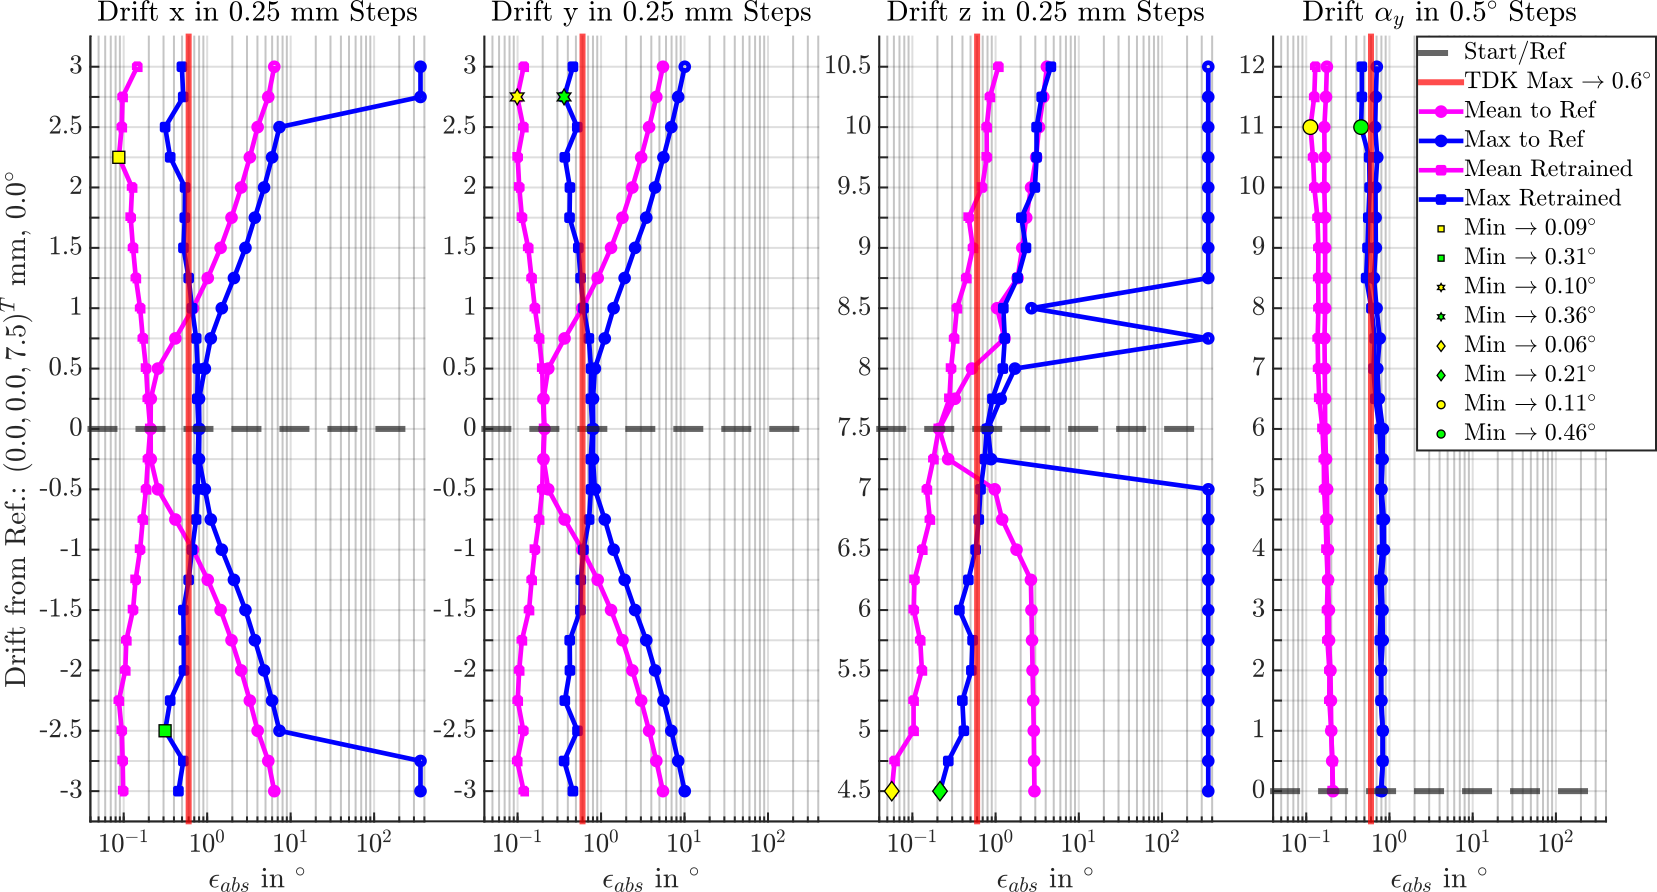
\includegraphics[width=.8\linewidth]{chapters/images/4-EuOExp/Drift-Model-Errors}
	\caption[Positionsdrift mit einfachen Versatz und Verkippung]{Positionsdrift mit einfachen Versatz und Verkippung. Simuliert sind Verschiebungen des Sensors entlang der $X-$, $Y-$ und $Z$-Achse des Koordinatensystem und Verkippung des Magneten in seiner $Y$-Achse, ausgehend von einer Referenz- bzw. Startposition bei $(0;0;7,5)^T$ mm und eine Magnetverkippung in der $Y$-Achse von $\SI{0}{\degree}$. Bei Verkippung des Magneten befindet sich der Sensor auf der Referenzposition. Es wird immer nur ein Drift z.Z. ausgeführt. Die Ausführung aller Drifte ist sequentiell. Für jeden Drift sind der mittlere und maximale absolute Winkelfehler aufgezeichnet worden. Es sind zwei Regressionsmodelle gleicher Konfiguration nach \autoref{eq:de2innorm} und \autoref{eq:kfun} als mittlerwertfreie Modelle zur Berechnung der Fehler genutzt worden. Das erste Modell ist einmalig auf der Referenzposition trainiert worden. Das zweite Modell ist bei jeder Driftposition trainiert worden (Retrained). Es ist zusätzlich der maximale Winkelfehler des TDK TMR-Sensors aufgetragen \cite{TDK2016}. Minimum der mittleren Fehler sind gelb markiert. Minimum der maximalen Fehler sind grün hervorgehoben.}
	\label{fig:drift-model-errors}
\end{figure}
\end{landscape}


\clearpage
\begin{landscape}
\begin{figure}[tbph]
	\centering
	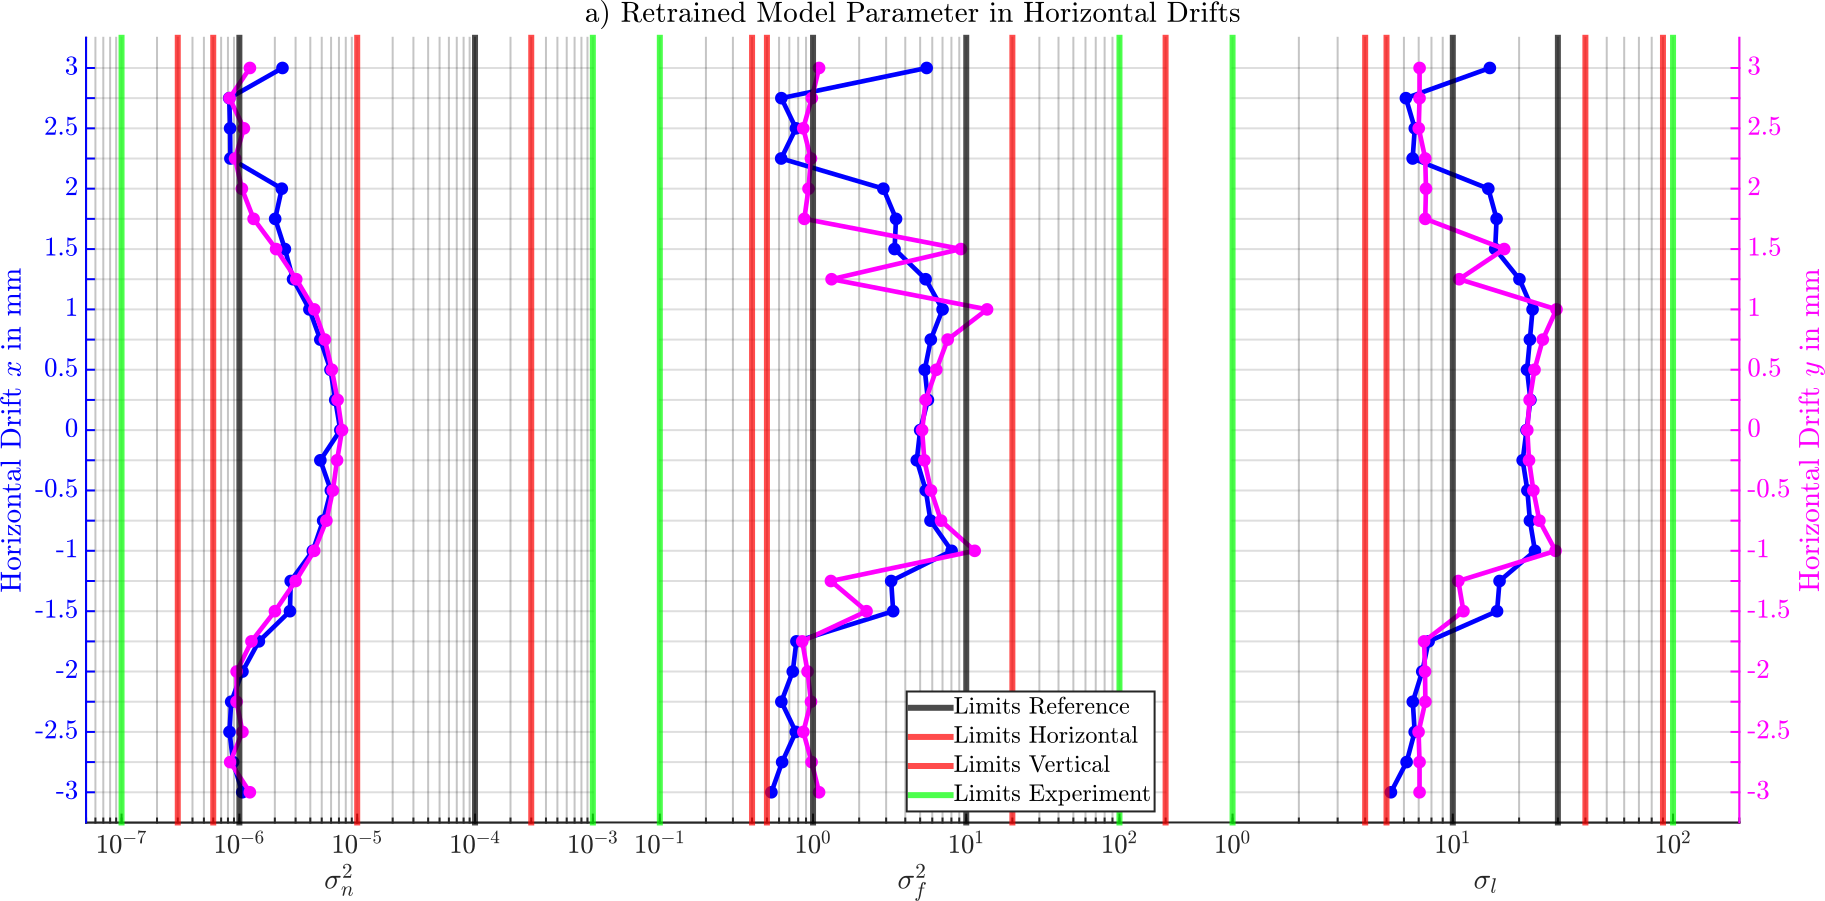
\includegraphics[width=\linewidth]{chapters/images/4-EuOExp/Drift-Horizontal-Model-Parms}
	\caption[Modellparameter bei horizontalem Drift]{Modellparameter bei horizontalen Drift. Aufgenommen sind das Rauschniveau $\sigma_n^2$ und die Höhenskalierung $\sigma_f^2$ sowie die Längenskalierung $\sigma_l$ der Kovarianzfunktion für das zweite Regressionsmodell (Retrained) aus \autoref{fig:drift-model-errors}, hier für Verschiebungen entlang der $X$-/ $Y$-Achse. Es sind Parametergrenzen als Referenz in Bezug auf Anpassungen aus \autoref{sec:exp4} aufgetragen. Zusätzlich sind die im Experiment genutzten Grenzen aufgetragen, sowie die sich hier ergebenen Grenzen aus horizontaler Verschiebung und die aus vertikaler Verschiebung bzw. Verkippung resultierenden Parametergrenzen aus \autoref{fig:drift-vertical-model-parms}.}
	\label{fig:drift-horizontal-model-parms}
\end{figure}
\end{landscape}


\clearpage
\begin{landscape}
	\begin{figure}[tbph]
		\centering
		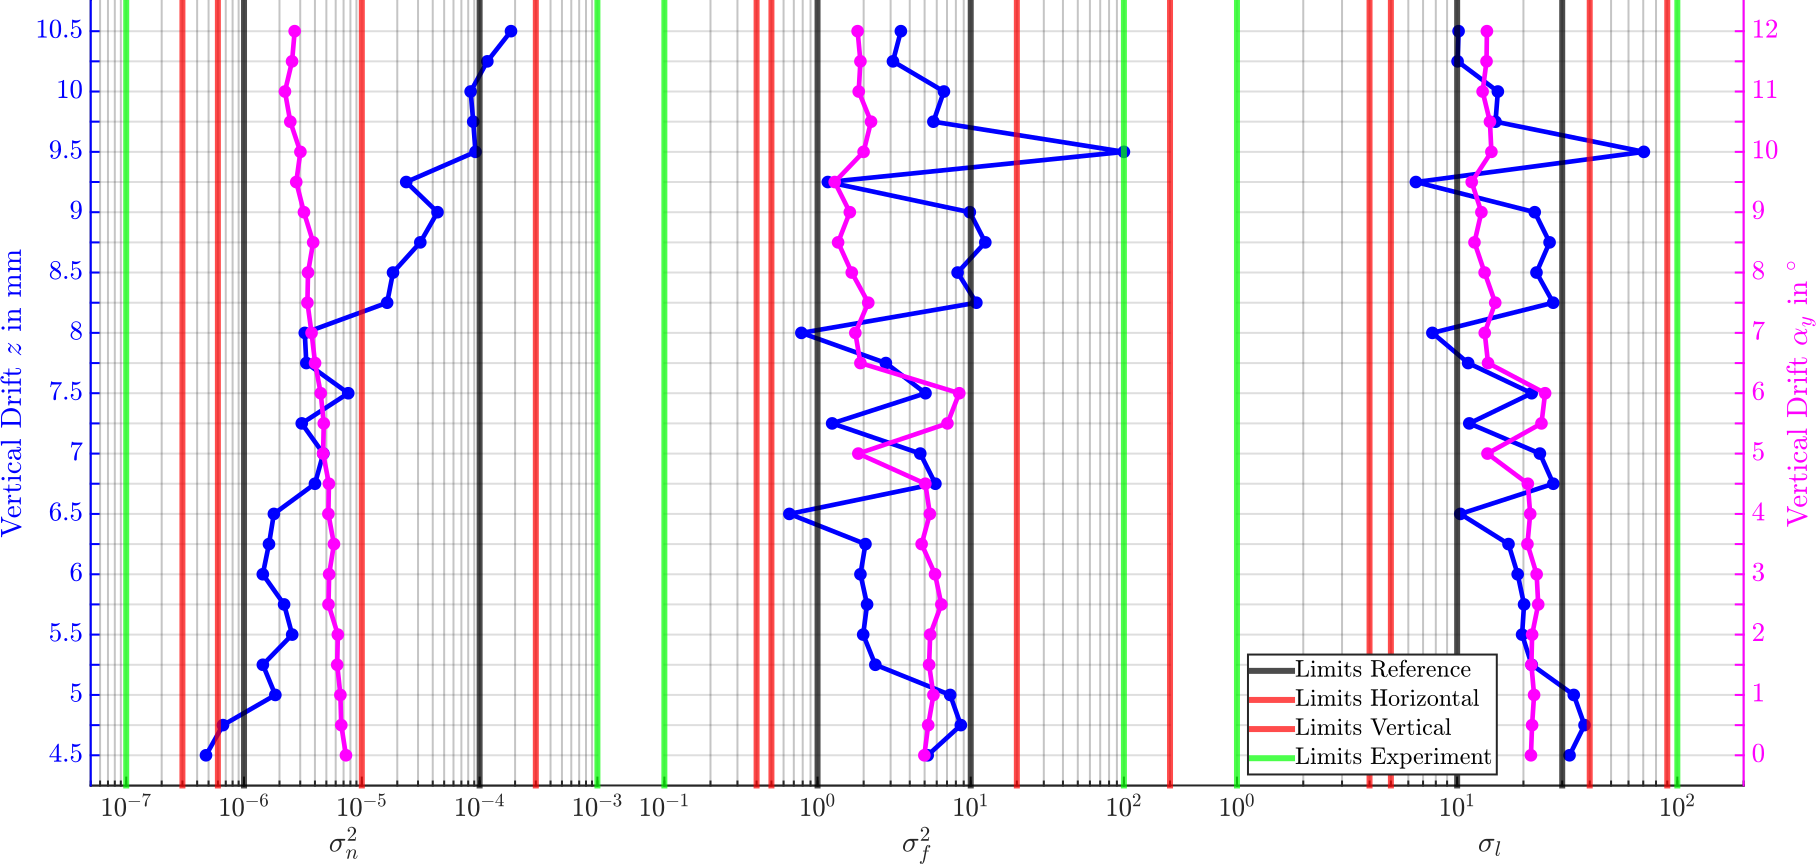
\includegraphics[width=\linewidth]{chapters/images/4-EuOExp/Drift-Vertical-Model-Parms}
		\caption[Modellparameter bei vertikalem Drift und Verkippung]{Modellparameter bei vertikalen Drift und Verkippung. Aufgenommen sind das Rauschniveau $\sigma_n^2$ und die Höhenskalierung $\sigma_f^2$ sowie die Längenskalierung $\sigma_l$ der Kovarianzfunktion für das zweite Regressionsmodell (Retrained) aus \autoref{fig:drift-model-errors}, hier für Verschiebungen entlang der $Z$-Achse und Verkippung des Magneten in der $Y$-Achse. Es sind Parametergrenzen als Referenz in Bezug auf Anpassungen aus \autoref{sec:exp4} aufgetragen. Zusätzlich sind die im Experiment genutzten Grenzen aufgetragen, sowie die sich hier ergebenen Grenzen aus vertikaler Verschiebung bzw. Verkippung und die aus horizontaler Verschiebung resultierenden Parametergrenzen aus \autoref{fig:drift-horizontal-model-parms}.}
		\label{fig:drift-vertical-model-parms}
	\end{figure}
\end{landscape}


\clearpage
\begin{figure}[tbph]
	\centering
	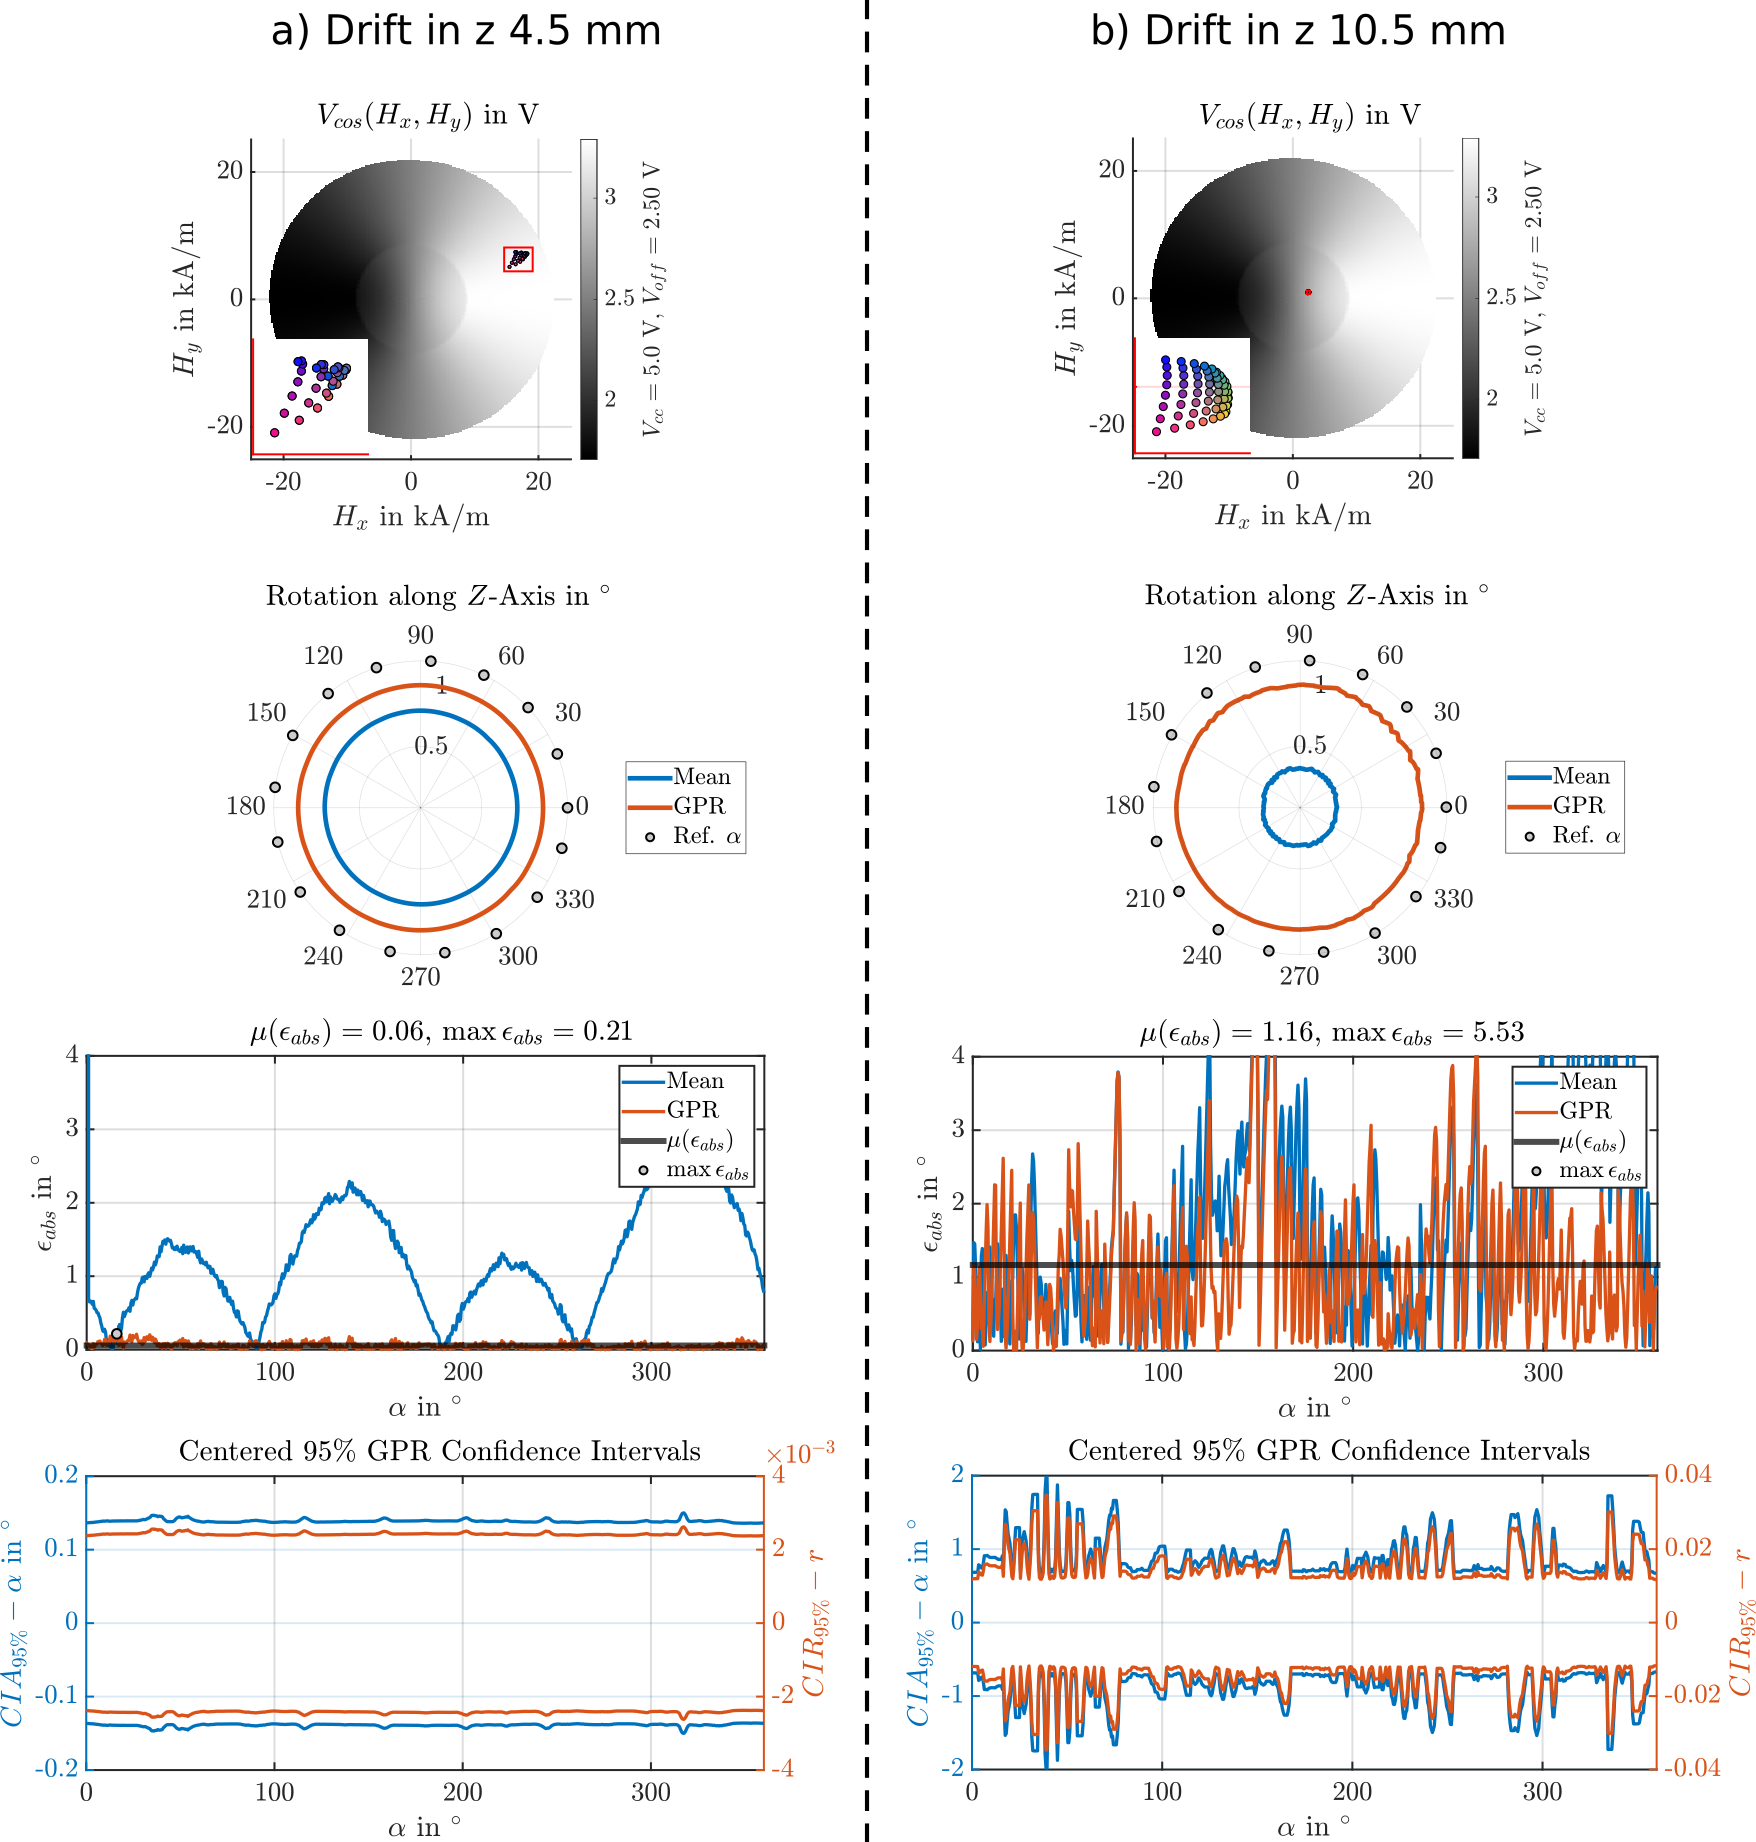
\includegraphics[width=\linewidth]{chapters/images/4-EuOExp/Z-Pos-Comp-45-105-Rotation}
	\caption[Best- und Worst-Case-Beispiel bei vertikalem Drift]{Best- und Worst-Case-Beispiel für vertikalem Drift aus \autoref{fig:drift-model-errors} für das zweite Regressionsmodell (Retrained). In a) und b) bei lotrechten und zentrierten Abstand vom Magneten ohne Verkippung. In a) mit $\SI{0,45}{\milli\metre}$ und in b) mit $\SI{10,5}{\milli\metre}$ Abstand. Für beide Beispiele ist die Sensor-Pixel-Streuung bei $\SI{21,5}{\degree}$ anhand des Kennfeldes für die Cosinus-Funktion gezeigt, sowie der Rotationsverlauf um die $Z$-Achse in Polardarstellung mit einfacher Mittlung der Daten (Mean) und Ergebnis via Gauß-Prozess-Regression (GPR) inklusive der Referenzwinkel für die GPR. Anschließend ist für beide Beispiele der absolute Winkelfehler über die volle Rotation aufgetragen mit nachfolgenden $95\%$ Konfidenzintervallen für Winkelvorhersagen (CIA) und Radius (CIR). Modelltrainingsdaten basieren auf Vektoren bzw. Skalare.}
	\label{fig:z-pos-comp-45-105-rotation}
\end{figure}


\clearpage


% !TEX root = ../thesis.tex
% testing and optimization experiments
% @author Tobias Wulf
%

\section{Verhalten bei kombinierten Fehllagen}\label{sec:exp6}

\textbf{Zweck:} Das Experiment soll als Stichprobe dienen und zeigen, dass das Regressionsmodell auch bei kombinierten Fehllagen funktionieren kann. Dafür werden eine Kombination der Parametergrenzen aus dem vorangegangenen Experiment aus \autoref{sec:exp5} übernommen, siehe \autoref{fig:drift-horizontal-model-parms} und \autoref{fig:drift-vertical-model-parms}. So setzt sich für das Rauschniveau $\sigma_n^2$ die Parametergrenzen aus der unteren Grenze für vertikalen Drift und oberen Grenze für horizontalen Drift zusammen. Für die Skalierungsparameter der Kovarianzfunktion, sind die Parametergrenzen aus horizontalem Drift für die Höhenskalierung $\sigma_f^2$ eingestellt. Die Längenskalierung $\sigma_l$ übernimmt ebenfalls die resultierenden Grenzen aus horizontalem Drift. Es sind wieder $N_{Ref} = 17$  Referenzwinkeln für das Regressionsmodell mit euklidischer Abstandsfunktion nach \autoref{eq:de2innorm} und resultierender Kovarianzfunktion nach \autoref{eq:kfun} vorgegeben. Das Modell wird als mittwertfreier Kernel betrieben. Die Durchlaufzahl für die äußere Optimierung nach \autoref{alg:bayesopt} ist mit $10$ Durchläufen wieder verringert. Modelltrainingsdaten basieren auf Vektoren bzw. Skalare.

\textbf{Durchführung:} Das Experiment wird in zwei Durchgängen ausgeführt. Vor jedem Durchgang werden Trainings- und Testdatensatz separat prozessiert und anschließend im Demonstrationsskript geladen. Es wird der Testdatensatz über einfache Mittlung der Daten ausgewertet. Die einfache Mittlung ist vom etwaigen Offset in den Simulationsdaten bereinigt. Es folgt die volle Regressionsmodell-Initialisierung und -Optimierung mittels Trainings- und Testdaten. Danach werden basierend auf den Testdaten die Vorhersage- und Verlust- sowie Fehlerberechnungen ausgeführt. Abschließend sind die Ergebnisse aus Regression und einfacher Mittlung grafisch ausgewertet. Die Testdaten beinhalten in jedem Durchgang $720$ Simulationswinkel bei einer Auflösung von $\SI{0,5}{\degree}$ und bilden eine volle Rotation des Magneten ab. Der Magnet ist in beiden Durchgängen um $\SI{11}{\degree}$ in der $Y$-Achse verkippt. Der $Z$-Abstand beträgt in beiden Durchgängen $4,5$ mm. Im ersten Durchgang ist der Sensor in $X$ um $0,5$ mm und in $Y$ um $1$ mm so verschoben, sodass sich der Magnet noch oberhalb des Sensors befindet. Beim zweiten Durchgang wird der Versatz in $X$ mit $2,5$ mm und für $Y$ mit $2$ mm nochmals erhöht. Der Magnet mit $2$ mm Radius liegt damit räumlich neben dem Sensor.

\textbf{Erzeugte Datensätze:} Jeweils zwei Trainings- und Testdatensätze mit korrespondierenden Positionen des Sensors und Verkippungswinkel des Magneten.

\textbf{Matlab-Skript:} demoGPRModule.m, siehe \autoref{mcode:demogprmodule}.


\clearpage


\textbf{Abweichende Parameter von \autoref{tab:sim-params-exp}:}

\begin{itemize}
	\item TrainingsOptions: nAngles: 17
	\item TrainingsOptions/ TestOptions: (xPos; yPos; zPos): 
	\begin{itemize}
		\item[a.] $(0,5;1;4,5)$
		\item[b.] $(2,5;2;4,5)$
	\end{itemize}
	\item TrainingsOptions/ TestOptions: tilt: $11$
	\item GRPOptions: kernel : 'QFCAPX'
	\item GRPOptions: $\sigma_f^2$-Bounds: $(0.4,20)$
	\item GRPOptions: $\sigma_l$-Bounds: $(4,40)$
	\item GRPOptions: $\sigma_n^2$-Bounds: $(3\cdot10^{-7},10^{-5})$
	\item GPROptions: mean: 'zero'
	\item GRPOptions: OptimRuns: 10
\end{itemize}

\textbf{Ergebnisse:} Die Ergebnisse beider Durchgänge sind in \autoref{fig:kombinierte-fehllagen-gpr} und \autoref{fig:kombinierte-fehllagen-sensor} grafisch gegenübergestellt. \autoref{fig:kombinierte-fehllagen-gpr} zeigt die Reaktion des Regressionsmodells und resultierende absolute Winkelfehler auf die kombinierten Fehllagen aus räumlichen Versatz und Verkippung des Magneten. Als ergänzende Darstellung zeigt \autoref{fig:kombinierte-fehllagen-sensor} die Reaktion des Sensor-Arrays in Bezug auf die gezeigten Beispiele in \autoref{fig:kombinierte-fehllagen-gpr}.


\clearpage


\textbf{Beobachtungen:} Für die Fehllage a) in \autoref{fig:kombinierte-fehllagen-gpr} zeigt sich, dass das Regressionsmodell diese sehr gut kompensieren konnte. Die Kovarianzmatrix zeigt ein homogenes Funktionsabbild für jeden Trainingspunkt zueinander mit nur sehr kleinen Abweichungen. Der Matrixmittelwert liegt mittig zu den einzelnen Kurvenverläufen. Die Kurvenverläufe besitzen eine gleichmäßige nicht spitz zulaufende Glockenform. Das Verhältnis aus Höhen- und Längenskalierung der Kovarianzfunktion liegt ca. bei $1:10$. Das Rauschniveau ist in der Optimierung gegen seine unter Parametergrenze gelaufen. Jedes Training-Sample hat dadurch annähernd den gleichen Einfluss in der Regression. Das Modell besitzt in Bezug auf die Trainingsdaten und unter Berücksichtigung des Parameterverhältnisses eine mittlere Komplexität \cite{Rasmussen2006}. Es stellt sich eine hohe Generalisierung mit $MSLLA$ und $MSLLR$ kleiner $-5$ ein. Es gibt leichte Schwankungen in der Generalisierung und zwei markante Ausreißer, die aber alle negativ sind und somit wenig bis mäßig vom Generalisierungniveau abweichen. Die Vorhersage ist sehr vertrauensvoll über die gesamte Rotation hinweg mit annähernd konstanten sehr engen Konfidenzintervallen für die Winkelvorhersage und Radius. Leichte Schwankungen in den Konfidenzintervallen entsprechen den Schwankungen der Modellverluste. Der mittlere Winkelfehler geht mit $\SI{0,4}{\degree}$ gegen null. Der maximale Winkelfehler ist mit $\SI{0,17}{\degree}$ sehr klein und taucht an der Peak-Stelle des Generalisierungsausreißers bei ca. $\SI{220}{\degree}$ auf. In der ergänzenden Ergebnisansicht in \autoref{fig:kombinierte-fehllagen-sensor} a) zeigt die polare Darstellung der Simulationsergebnisse, dass die einfache Mittlung der Daten zwar eine Kreisbahn ergibt, diese aber nicht zentriert ist. Das Regressionsmodell gleicht diese Fehllage vollständig aus. Die Streuung der Sensor-Pixel auf dem Kennfeld deckt annähernd den vollen nichtlineare Bereich des Kennfeldes ab. Die Sensor-Pixel überlagern sich teilweise. Das Sensor-Pixel mit der Koordinate $(1,8)$ liegt dabei an der Grenze zum linearen Bereich des Kennfeldes. Die Auswertung der einzelnen Sensor-Pixel-Kreisbahnen zeigen, dass sich erste Darstellungsprobleme an der Sensor-Pixel-Koordinate $(1,8)$ und angrenzende Pixel einstellen. Hervorgerufen durch die stärkere Verzerrung der Feldstärkenverläufe von Kreisbahnen zu Ellipsoiden.
\newline
Mit der Fehllage b) in \autoref{fig:kombinierte-fehllagen-gpr} hat das Regressionsmodell Schwierigkeiten diese zu kompensieren. Das Skalierungsverhältnis von Höhen- zu Längenparameter liegt ca. bei $7:50$. Die Kurvenverläufe sind stark inhomogen und  sind wechselhaft zwischen breiten Glocken- und Keilformen. Der Matrixmittelwert ist abgesenkt. In Bezug auf die Trainingsdaten und Parameterverhältnis stellt sich damit z.T. eine hohe Modellkomplexität ein, die für einige Trainingsdaten durch keilförmige Kurven durchbrochen ist  \cite{Rasmussen2006}. Mit einfachen Worten, das Regressionsmodell kann sich nicht auf die stark variierenden Daten einstellen, sodass der versuchte Kompromiss in der Komplexität fehlschlägt. Das Generalisierungsniveau ist negativ und von der Mittlung bei ca. $-4$ zufriedenstellend, allerdings abschnittsweise in Gänze aufgehoben, sodass nur der Fit auf den Trainingsdaten erhalten bleibt. Die Ursache dafür ist die Keilform an den jeweiligen Trainingsdatenpunkten in der Kovarianzmatrix. Der Bruch in der Generalisierung ist zwischen $\SI{0}{\degree}$ und $\SI{110}{\degree}$ sowie zwischen $\SI{150}{\degree}$ und $\SI{275}{\degree}$ zu beobachten. Gleichmaßen zeigen sich Einbußen für die Generalisierung in der Vertrauensaussage über die Konfidenzintervalle wieder. Dies ist durch ein Aufschwingen der Intervalle in den angegebenen Abschnitten zu sehen. Der Winkelfehler folgt entsprechend der Generalisierung und dem Konfidenzintervall. Der mittlere Fehler hat sich erhöht auf $\SI{0,33}{\degree}$, der maximale liegt nun bei rund $\SI{2}{\degree}$. Die Ergänzung in \autoref{fig:kombinierte-fehllagen-sensor} b) zeigt die Verzerrung der Testdaten in einfacher Mittlung zu einer nicht kreisförmigen oder ellipsenähnlichen Bahn führen. Das Regressionsmodell schafft es nicht die stark verzerrte Kreisbahn zu kompensieren. Die Sensor-Pixel-Ansicht auf dem Cosinus-Kennfeld zeigt, dass die Pixel-Überlagerung vollständig aufgehoben ist und die Streuung der Pixel vom nichtlinearen Kennfeldbereich über den lineare bis hin zur Kennfeldmitte nahe $\SI{0}{\kilo\ampere\per\metre}$ reicht. Die jeweiligen Feldstärkenverläufe sind alle zu Ellipsen gestaucht und werden im Bereich der Sensor-Pixel-Koordinate $(1,8)$ so stark gestaucht, dass sie nun mehr als Linien wahrnehmbar sind. Das resultiert für die Betrachtung der Ausgangsspannungen zu stark verzerrten und größtenteils nicht kreis- oder ellipsenförmigen Bahnverläufen.


\clearpage
\begin{figure}[tbph]
	\centering
	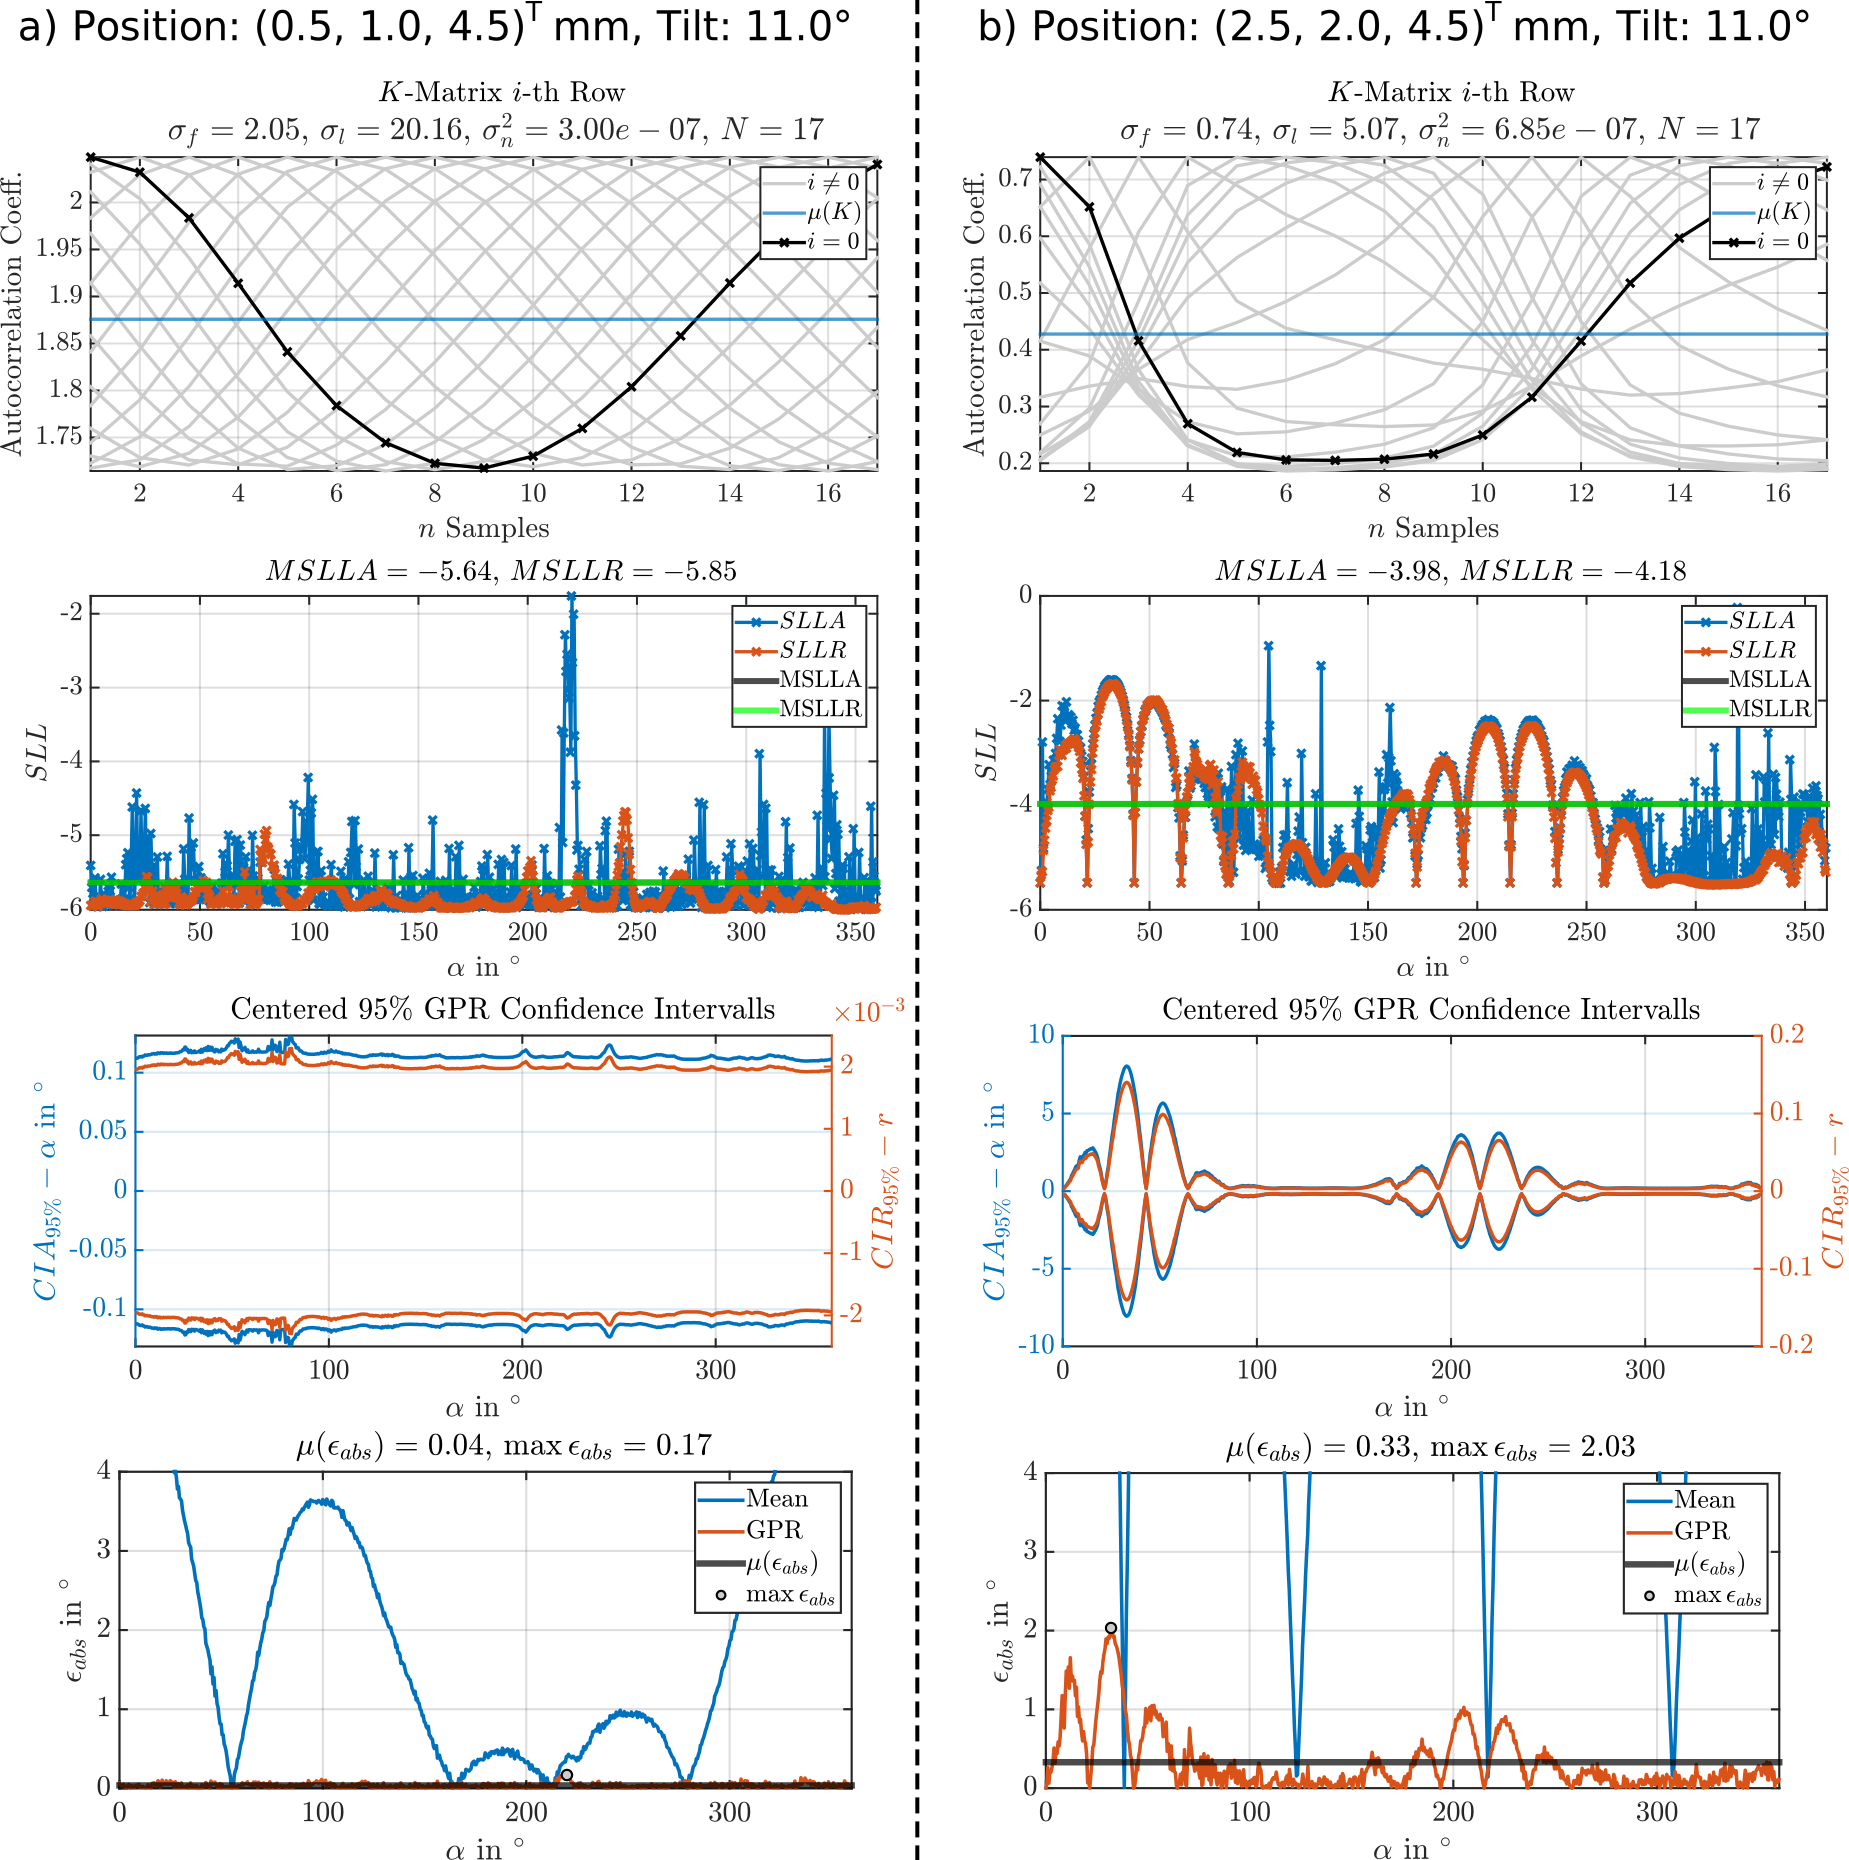
\includegraphics[width=\linewidth]{chapters/images/4-EuOExp/Kombinierte-Fehllagen-GPR}
	\caption[Beispiel kombinierter Fehllagen in der Regressionsansicht]{Beispiel kombinierter Fehllagen in der Regressionsansicht. Gezeigt sind zwei Fehllagen mit gleicher Magnetverkippung und $Z$-Abstand zum Magneten. Für a) befindet sich der Magnet räumlich über den Sensor. Für b) liegt der Sensor räumlich neben dem Magneten. Der Magnetradius beträgt $2$ mm. Beide Beispiele sind mit voll optimierten Modell nach \autoref{alg:fminconopt} und \autoref{alg:bayesopt} und gleicher Konfiguration ausgeführt worden. Genutzt ist der Kernel nach \autoref{eq:kfun} mit Abstandsfunktion nach \autoref{eq:de2innorm}. Die Referenzwinkelanzahl beträgt $N_{Ref} = 17$. Gezeigt sind: Die Kovarianzmatrix aufgetragen für jede $i-te$ Matrixreihe inklusive Matrixmittelwert. Die Generalisierung über den standardisierten logarithmischen Verlust (engl. Loss) $SLL$, jeweils für Winkel $SLLA$ und Radius $SLLR$, sowie die resultierende Verlustmittlung $MSLLA$ und $MSLLR$. Die $95\%$ Konfidenzintervalle aus Winkelvorhersage $CIA_{95\%}$ und Radius $CIR_{95\%}$. Der absolute Winkelfehler durch Mittlung (Mean) und Gauß-Prozess-Regression (GPR).}
	\label{fig:kombinierte-fehllagen-gpr}
\end{figure}


\clearpage
\begin{landscape}
\begin{figure}[tbph]
	\centering
	\includegraphics[width=.85\linewidth]{chapters/images/4-EuOExp/Kombinierte-Fehllagen-Sensor}
	\caption[Beispiel kombinierter Fehllagen aus Sicht des Sensor-Arrays]{Beispiel kombinierter Fehllagen aus Sicht des Sensor-Arrays. Ergänzung zur \autoref{fig:kombinierte-fehllagen-gpr}. Die Fälle a) und b) korrespondieren zu den gezeigten Beispielen in \autoref{fig:kombinierte-fehllagen-gpr}. Gezeigt sind: Die polare Darstellung aus einfacher Mittlung (Mean) der Testdaten und Ergebnis der Gauß-Prozess-Regression (GPR) inkl. Anzeige der Referenzwinkel. Das Streuungsmuster der Sensor-Pixel auf dem Kennfeld der Cosinus-Funktion für den Simulationswinkel $\alpha = \SI{21,5}{\degree}$. Die $H_x$- und $H_y$-Feldstärkenverläufe normiert auf die globale maximale Betragsfeldstärke $|H|$ aller simulierten Feldstärken. Die Simulationsergebnisse der Sensor-Array-Simulation für Cosinus- und Sinus-Ausgangsspannungen normiert auf das globale Betragsmaximum $|V|$, als resultierendes Betragsmaximum aller simulierten Ausgangsspannungen. Beide Ansichten zur Feldstärke und Spannung bilden die gleichen Sensor-Pixel-Positionen  bei voller Magnetrotation ab. Die Farbgebung entspricht der Pixel-Darstellung auf dem Kennfeld. Die Magnetposition ist in a) und b) rot hervorgehoben. In b) befindet das Sensor-Array neben dem Magneten, die Position ist daher nur angedeutet.}
	\label{fig:kombinierte-fehllagen-sensor}
\end{figure}	
\end{landscape}


\clearpage



